\documentclass[xcolor=dvipsnames,8pt,aspectratio=34]{beamer}
%\documentclass[xcolor=dvipsnames,10pt]{beamer}
\usepackage{etex}
\usepackage{pgf,pgfarrows,pgfnodes,pgfautomata,pgfheaps,pgfshade}
\usepackage[absolute,overlay]{textpos} 
%\usepackage{algorithm}
\usepackage{amsmath,amssymb}
\usepackage[utf8]{inputenc} 
\usepackage{colortbl}
\usepackage{graphicx} 
\usepackage[english]{babel}
\usepackage{tabularx} 
\usepackage{multirow}
\usepackage{booktabs}
\usepackage{listings}
%\usepackage{multimedia}
\usepackage{animate}
\usepackage{xcolor}
\usepackage{array}
\usepackage{longtable}
\usepackage{makecell}
\usepackage{caption}
\usetheme{Madrid} 
\usepackage{amsmath}
\usepackage{movie15}


\lstset{ %
%	backgroundcolor=\color{white},   % choose the background color; you must add \usepackage{color} or \usepackage{xcolor}
%	basicstyle=\footnotesize,        % the size of the fonts that are used for the code
	basicstyle=\scriptsize,        % the size of the fonts that are used for the code
	breakatwhitespace=false,         % sets if automatic breaks should only happen at whitespace
	breaklines=true,                 % sets automatic line breaking
	captionpos=t,                    % sets the caption-position to bottom
	commentstyle=\color{mygreen},    % comment style
	deletekeywords={...},            % if you want to delete keywords from the given language
	escapeinside={\%*}{*)},          % if you want to add LaTeX within your code
	extendedchars=true,              % lets you use non-ASCII characters; for 8-bits encodings only, does not work with UTF-8
%	frame=single,                    % adds a frame around the code
	keepspaces=true,                 % keeps spaces in text, useful for keeping indentation of code (possibly needs columns=flexible)
	keywordstyle=\color{blue},       % keyword style
%	language=make,                 % the language of the code
	morekeywords={*,...},            % if you want to add more keywords to the set
%	numbers=left,                    % where to put the line-numbers; possible values are (none, left, right)
%	numbersep=5pt,                   % how far the line-numbers are from the code
	numberstyle=\tiny\color{mygray}, % the style that is used for the line-numbers
	rulecolor=\color{black},         % if not set, the frame-color may be changed on line-breaks within not-black text (e.g. comments (green here))
	showspaces=false,                % show spaces everywhere adding particular underscores; it overrides 'showstringspaces'
	showstringspaces=false,          % underline spaces within strings only
	showtabs=false,                  % show tabs within strings adding particular underscores
	stepnumber=2,                    % the step between two line-numbers. If it's 1, each line will be numbered
}

\definecolor{mygreen}{rgb}{0,0.6,0}
\definecolor{mygray}{rgb}{0.5,0.5,0.5}
\definecolor{mymauve}{rgb}{0.58,0,0.82}

\usecolortheme{beaver}
\newcommand{\ul}{\underline}
\setbeamertemplate{footline}{\scriptsize{\vspace*{0.3cm}\hspace*{15cm}\insertframenumber\,/\,\inserttotalframenumber}}
\setbeamertemplate{caption}[numbered]
\setbeamerfont{caption}{size=\fontsize{8}{5}}

\setbeamercolor{block title}{	bg=Sepia , fg = White}
\setbeamercolor{block body}{bg=Brown!15, fg=Sepia }
\setbeamercolor{item projected}{bg=Sepia, fg=White}
\setbeamercolor{number projected}{bg = Black}

%declara as imagens usadas no layout do slide
\pgfdeclareimage[height=0.8cm]{mflab}{figuras/logo_mflab_transparente.png}
\pgfdeclareimage[height=1.0cm]{logoufu}{figuras/logo_ufu.jpg}
\pgfdeclareimage[height=1.0cm]{petro}{figuras/EPTT.jpg}

%posiciona o logotipo do MFLab
\setlength{\TPHorizModule}{1mm}
\setlength{\TPVertModule}{1mm}
\newcommand{\placelogomflab} 
{ 
	\begin{textblock}{13}(150.0,0.0)
		\pgfuseimage{mflab} 
	\end{textblock} 
	
% 	\begin{textblock}{13}(128.0,1.0)
% 		\pgfuseimage{logoufu} 
% 	\end{textblock} 
	
	\begin{textblock}{13}(150.0,70.0)
		\pgfuseimage{petro} 
	\end{textblock} 
}
%posiciona o logotipo do MFLab
\setlength{\TPHorizModule}{1mm}
\setlength{\TPVertModule}{1mm}
\newcommand{\placelogo} 
{ 
	\begin{textblock}{13}(150.0,0.0)
		\pgfuseimage{mflab} 
	\end{textblock} 
	
% 	\begin{textblock}{13}(128.0,1.0)
% 		\pgfuseimage{logoufu} 
% 	\end{textblock} 
	
	\begin{textblock}{13}(0.0,80.0)
		\pgfuseimage{petro} 
	\end{textblock} 
}

% \setlength{\TPHorizModule}{1mm}
% \setlength{\TPVertModule}{1mm}
% \newcommand{\placelogomflab_titulo} 
% { 
% 	\begin{textblock}{13}(150.0,0.0)
% 		\pgfuseimage{mflab} 
% 	\end{textblock} 
% 	
% 	\begin{textblock}{13}(0.0,0.0)
% 		\pgfuseimage{lmest} 
% 	\end{textblock} 
% 	
% % 	\begin{textblock}{13}(128.0,1.0)
% % 		\pgfuseimage{logoufu} 
% % 	\end{textblock} 
% 	
% 	\begin{textblock}{13}(75.0,80.0)
% 		\pgfuseimage{petro} 
% 	\end{textblock} 
% }



%insere o logotipo da ufu em todos os slides
% \logo{
\includegraphics[height=0.8cm]{figuras/layout_slide/petrobras.png}}

\title{Theoretical analyze of turbulent channel flow with thermal effects - the influence of the turbulent Prandtl number}

\author{ Felipe J. O. Ribeiro \\ \and \\ Prof. Dr. Aristeu da Silveira Neto}

%\date{\tiny{02 de dezembro de 2015}}
\date{\tiny{\today}}
% \newcolumntype{M}[1]{>{\raggedright\arraybackslash}b{#1}}
% \newcolumntype{N}{@{}m{0pt}@{}}	
% \newcolumntype{M}{>{\begin{minipage}[b]{3cm}\raggedright{}}c<{\end{minipage}\minrowheight}}
% \setlength\extrarowheight{5pt}
\newcolumntype{C}[1]{>{\centering\let\newline\\\arraybackslash\hspace{0pt}}m{#1}}


\begin{document}

	\begin{frame}\placelogomflab
		\frametitle 
		{ \vfill
			\centering
			{
			\small{Federal university of Uberlandia}\\
%			\small{Programa de Pós-Graduação em Engenharia Mecânica}\\
			\small{Fluids Mechanical laboratory}\\
			}
		}
		\maketitle
	\end{frame}

	\section<presentation>*{Summary}


		\AtBeginSection[]
		{
		 \begin{frame}<beamer>
		  \frametitle{Summary}\placelogomflab 
		  {\scriptsize \tableofcontents[current,currentsection]}
		 \end{frame}
		}

		\AtBeginSubsection[]
		{
		 \begin{frame}<beamer>
		  \frametitle{Summary}\placelogomflab 
		  {\scriptsize \tableofcontents[current,currentsubsection]}
		 \end{frame}
		}


	\section{Introduction}
	
	
	
	
	
	
		\begin{frame}
		\frametitle{Analysis of turbulent plane Poiseuille flows}
			\begin{minipage}[h!]{0.49\textwidth}
			$\bullet$ The study of thermal behavior of flows is of great importance to current scientific development. As industrial machinery is improved, so does the world's energy consumption. Much of this cost arises from the energy transformations within the system, mostly resulting in thermal manifestations. Thus a great need for thermal management mechanisms arises. Since diffusion is a very slow process, the most used medium for cooling industrial machinery is the advective behavior, where a fluid-structure interface carries thermal energy out of the system. Studying these phenomena is essential for more and more efficient machines, thus ensuring sustainable development. 
		\end{minipage}
		\begin{minipage}[h!]{0.49\textwidth}
			\begin{figure}[h!]
				\centering
				
\includegraphics[trim = {1.7cm 2cm 0 1cm}, clip , angle=0, scale=0.40]{turbulence}
				\caption{Temperature and turbulence.}
			\end{figure}
		\end{minipage}
		\end{frame}





	\section{Physical model}
	
	
	
	
	
		\begin{frame}
			\frametitle{Plane Poiseuille flow}
			$\bullet$ The problem was defined as a channel flow, with only one finite dimension $y$. \\
			$\bullet$ The boundary conditions were determined as two infinite plates in a constant thermal flux regime.\\
			$\bullet$ A constant pressure gradient was imposed on the $x$ axis.\\
			$\bullet$ A dynamic and thermal self similarity was proposed in the $z$ axis, resulting in a dynamic one-dimensional problem and a two-dimensional thermal analysis (Fig.\ref{figure.1}). \\
			$\bullet$ Incompressible flows of Newtonian fluid in a turbulent regime.\\
			\begin{minipage}[h!]{0.3\textwidth}
				\begin{equation*}
				 \frac{\partial T }{\partial z} = 0.
				\end{equation*}
				\begin{equation*}
				\frac{\partial u }{\partial z} = 0.
				\end{equation*}
				\begin{equation*}
				\frac{\partial u }{\partial x} = 0.
				\end{equation*}
			\end{minipage}
			\begin{minipage}[h!]{0.5\textwidth}
			\begin{figure}[h!]
				\centering
				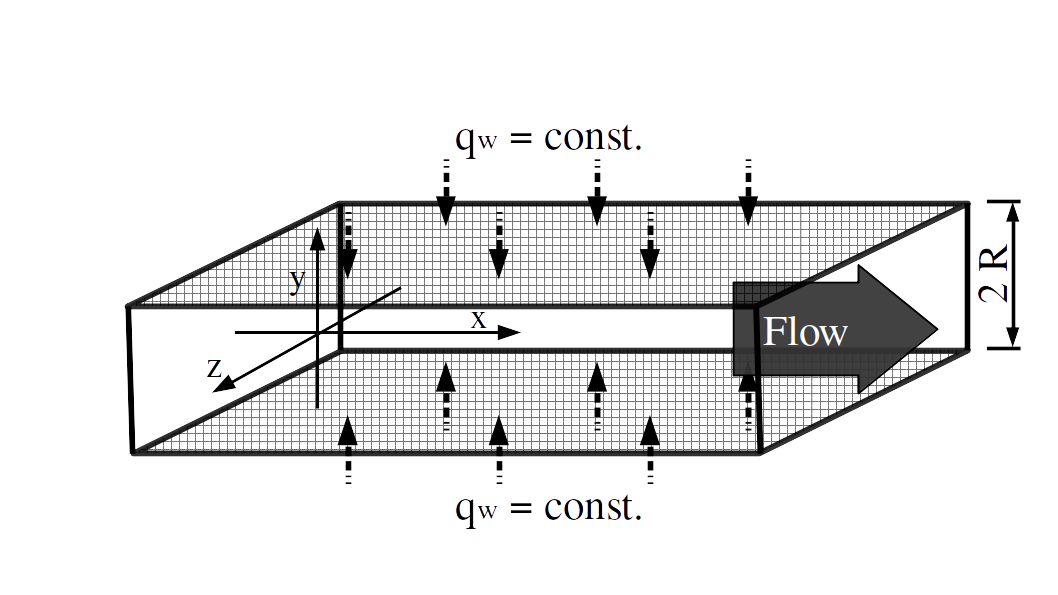
\includegraphics[trim={2.0 0.5 0.5 0.5}, angle=0, clip , scale=0.30]{fotos_formatacao_final/canal1}
				\caption{Geometric definition, and boundary conditions.}
				\label{figure.1}
			\end{figure}
			\end{minipage}
			\\
		\end{frame}
	
	

	
	\section{Differential Mathematical Model}
	
	
	
	
		
%		\begin{frame}
%		\frametitle{Equações do movimento}
%		$\bullet$ Para modelar diferencialmente a velocidade do fluido, foram utilizadas a equação da continuidade e a equação de Navier-Stokes para a velocidade no eixo de interesse.
%		\begin{equation}
%		\frac{\partial u}{\partial t} + \frac{\partial u^2}{\partial x} + \frac{\partial uv}{\partial y} + \frac{\partial uw}{\partial z} = - \frac{1}{\rho} \frac{\partial {p}}{\partial x} + \nu \left( \frac{\partial^2 u}{\partial x^2} + \frac{\partial^2 u}{\partial y^2} + \frac{\partial^2 u}{\partial z^2}   \right)
%		\end{equation}
%		\begin{equation}
%		\frac{\partial \rho}{\partial t} +  \frac{\partial (\rho u)}{\partial x} + \frac{\partial (\rho v)}{\partial y} + \frac{\partial (\rho w)}{\partial z} = 0
%		\end{equation}
%		Para o desenvolvimento da equação da energia em uma instancia convectiva foi necessário o desenvolvimento do perfil cinético do sistema.
%		\end{frame}

		



		\begin{frame}
		\frametitle{Thermal energy balance equation}
		$\bullet$ Was utilize the thermal energy balance equation.
		\begin{equation}
		\frac{\partial T}{\partial t} + {\frac{\partial{}}{\partial{x}} (uT)} + {\frac{\partial{}}{\partial{y}} (vT)} + {\frac{\partial{}}{\partial{z}} (wT)}
		=
		{\frac{\partial{}}{\partial{x}}} \left(\alpha {\frac{\partial{T}}{\partial{x}}} \right) +
		{\frac{\partial{}}{\partial{y}}} \left(\alpha {\frac{\partial{T}}{\partial{y}}} \right) +
		{\frac{\partial{}}{\partial{z}}} \left(\alpha {\frac{\partial{T}}{\partial{z}}} \right) .
		\end{equation}
		$ $
		$\bullet$ Being necessary this definition for nondimensionalization.
		\begin{equation}\label{c_h_e}
		q_{conv.} = \dot{m} C_p \Delta T_m.
		\end{equation}
		$ $
		With these mathematical constructs it was possible to begin differential development.
		\end{frame}




		
		
		\begin{frame}
			\frametitle{Mean values principle}
			$\bullet$ 
			In order to proceed with the simplifications of the differential equations it was necessary to use the concepts of mean values. Such consideration implies the use of the RANS methodology. (Reynolds Averaged Navier Stokes)
			\\
			\begin{minipage}[h!]{0.45\textwidth}
				\begin{equation*}
				\label{ola}
				\text{Properties}=
				\begin{cases}
				\overline{f}({x})=\frac{1}{t_f - t_i} \int_{t_i}^{t_f} f({x} , t) dt.      & \quad  \\
				f({x} , t) = \overline{f}({x}) + f^\prime ({x} ,t) . & \quad   \\
				\overline{f^\prime ({x} ,t)} = 0 . & \quad   \\
				\overline{\overline{f({x})}} = \overline{f({x})} . & \quad   \\
				\overline{f^\prime ({x} ,t)\overline{f({x})}} = 0 .& \quad   \\
				\overline{f^\prime ({x} ,t)g^\prime ({x} ,t)} \neq 0 . & \quad   \\
				\overline{  \overline{g({x})} \ \overline{f({x})}  } = {\overline{g({x})}} \ {\overline{f({x})}} . & \quad   \\
				\end{cases}
				\end{equation*}
			\end{minipage}\hfill
			\begin{minipage}[h!]{0.45\textwidth}
				\begin{figure}
					\centering
					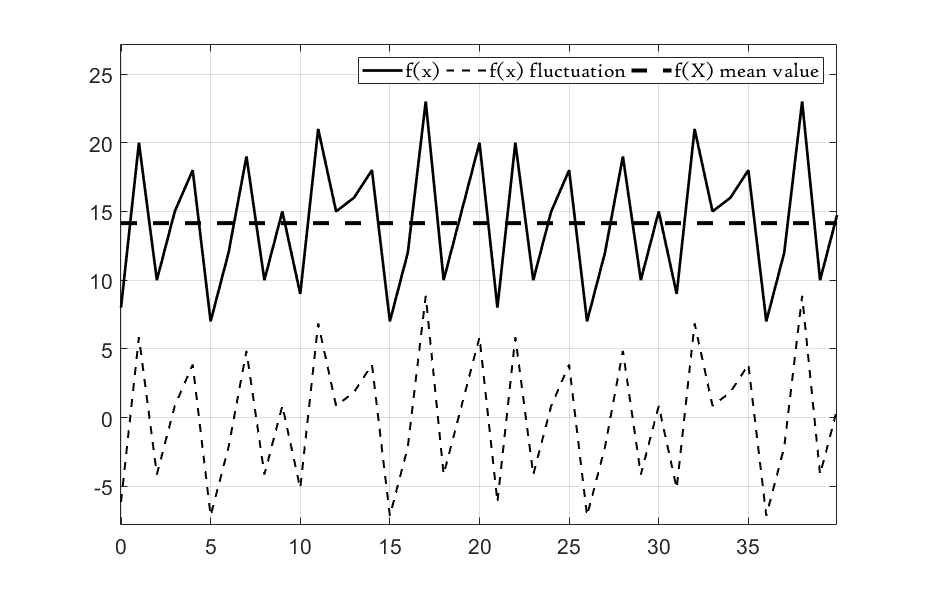
\includegraphics[angle=0, scale=0.22]{medios}
					\caption{Graphical representation of the concept.}
					\label{medios}
				\end{figure}
			\end{minipage}
	     	\\
		\end{frame}
	
	
	
	
	
		
%				\begin{frame}
%		\frametitle{Simplificando a velocidade para valores médios}
%		\begin{equation}
%		\frac{\partial \overline{u}}{\partial t} + \frac{\partial \overline{u^2}}{\partial x} + \frac{\partial \overline{uv}}{\partial y} + \frac{\partial \overline{uw}}{\partial z} = - \frac{1}{\rho}  \frac{\partial \overline{p}}{\partial x} + \nu  \left( \frac{\partial^2 \overline{u}}{\partial {x^2}} + \frac{\partial^2 \overline{u}}{\partial y^2} + \frac{\partial^2 \overline{u}}{\partial z^2}   \right)
%		\end{equation}
%		\\
%		\begin{equation}
%		\begin{split}
%		\frac{\partial \overline{(\overline{u} + u^\prime)}}{\partial t} + \frac{\partial \overline{(\overline{u}^2 + 2  \overline{u}  u^\prime + {u^\prime}^2)}}{\partial x} + \frac{\partial \overline{(\overline{u}\ \overline{v} + u^\prime  \  \overline{v} + \overline{u}  v^\prime + u^\prime  v ^\prime )}}{\partial y} + \\
%		\frac{\partial \overline{(\overline{u} \ \overline{w} + u^\prime  \overline{w} + \overline{u}  w^\prime + u^\prime  w ^\prime )}}{\partial z} = - \frac{1}{\rho}  \frac{\partial \overline{(\overline{p} + p ^\prime)}}{\partial x} + \nu  \left( \frac{\partial^2 \overline{(\overline{u} + u^\prime)}}{\partial {x^2}} + \frac{\partial^2 \overline{(\overline{u} + u^\prime)}}{\partial y^2} + \frac{\partial^2 \overline{(\overline{u} + u^\prime)}}{\partial z^2}   \right)
%		\end{split}
%		\end{equation}
%		\\
%		\begin{equation}
%		\begin{split}
%		\frac{\partial \overline{u}}{\partial t} + \frac{\partial \overline{u^2}}{\partial x} + \frac{\partial \overline{u} \ \overline{v}}{\partial y} + \frac{\partial \overline{u} \ \overline{w}}{\partial z} =  - \frac{1}{\rho}  \frac{\partial \overline{{p}}}{\partial x} + \frac{\partial}{\partial x} \left( \nu \frac{\partial \overline{u}}{\partial x} - \overline{{u^\prime}^2}\right) + \frac{\partial}{\partial y} \left( \nu \frac{\partial \overline{u}}{\partial y} - \overline{{u^\prime v^\prime}}\right) \\
%		+ \frac{\partial}{\partial z} \left( \nu  \frac{\partial \overline{u}}{\partial z} - \overline{ u ^\prime w ^\prime} \right)
%		\end{split}
%		\end{equation}
%		\end{frame}
		
		
		
		
		
%		\begin{frame}
%			\frametitle{Modelando a equação da continuidade para valores médios}
%			$\bullet$ Desenvolvendo a equação da Continuidade, é possível se chegar a uma conclusão muito importante, para os valores médios.
%			\begin{equation*}
%			\color{red}\frac{\partial \rho}{\partial t} \color{black}+  \frac{\partial (\color{red}\rho \color{black}u)}{\partial x} + \frac{\partial (\color{red} \rho \color{black}v)}{\partial y} + \frac{\partial (\color{red}\rho \color{black}w)}{\partial z} = 0
%			\end{equation*}
%			\begin{equation}
%			\frac{\partial u}{\partial x} + \frac{\partial v}{\partial y} + \frac{\partial w}{\partial z} = 0
%			\end{equation}
%			\begin{equation}
%			\frac{\partial \overline{(u^\prime + \overline{u})}}{\partial x} + \frac{\partial \overline{(v^\prime + \overline{v})}}{\partial y} + \frac{\partial \overline{(w^\prime + \overline{w})}}{\partial z} = 0
%			\end{equation}
%			\begin{equation}
%			\frac{\partial \overline{u^\prime}}{\partial x} +\frac{\partial \overline{\overline{u}}}{\partial x} + \frac{\partial \overline{v\prime}}{\partial y} +\frac{\partial \overline{\overline{v}}}{\partial y} + \frac{\partial \overline{w\prime}}{\partial z} +\frac{\partial \overline{\overline{w}}}{\partial z} = 0
%			\end{equation}
%			\begin{equation}
%			\frac{\partial {\overline{u}}}{\partial x} +\frac{\partial {\overline{v}}}{\partial y} +\frac{\partial {\overline{w}}}{\partial z} = 0
%			\end{equation}
%			Assim, como $ \frac{\partial {\overline{v}}}{\partial y} $ e $ \frac{\partial {\overline{w}}}{\partial z}$ são iguais a zero, por definição do comportamento médio dos escoamentos, necessariamente $\frac{\partial {\overline{u}}}{\partial x}$ deve ser igual a zero também, o que demonstra como o sistema resultante é unidimensional.
%		\end{frame}
%		
		
		
		
%		\begin{frame}
%		\frametitle{Simplifying the temperature to average values}
%		\begin{equation}
%		\frac{\partial \overline{T}}{\partial t} + {\frac{\partial{}}{\partial{x}} \overline{(u T)}} + 
%		{\frac{\partial{}}{\partial{y}} \overline{(v T)}} 
%		=
%		{\frac{\partial{}}{\partial{x}}} \left(\alpha {\frac{\partial{\overline{T}}}{\partial{x}}} \right) +
%		{\frac{\partial{}}{\partial{y}}} \left(\alpha {\frac{\partial{\overline{T}}}{\partial{y}}} \right) .
%		\end{equation}
%		\begin{equation}
%		\begin{split}
%		\frac{\partial \overline{(\overline{T} + T^\prime)}}{\partial t} +{\frac{\partial{}}{\partial{x}} \overline{\left((\overline{u} + u^\prime)  (\overline{T} + T^\prime) \right)}} + 
%		{\frac{\partial{}}{\partial{y}} \overline{(\left(\overline{v} + v^\prime)  (\overline{T} + T^\prime) \right)}} 
%		= \\
%		{\frac{\partial{}}{\partial{x}}} \left(\alpha {\frac{\partial{\overline{(\overline{T} + T^\prime)}}}{\partial{x}}} \right) +
%		{\frac{\partial{}}{\partial{y}}} \left(\alpha {\frac{\partial{\overline{(\overline{T} + T^\prime)}}}{\partial{y}}} \right) .
%		\end{split}
%		\end{equation}
%		\begin{equation}
%		\frac{\partial \overline{T}}{\partial t} +\frac{\partial{}}{\partial{x}} \left(\overline{\left({T^\prime u^\prime}\right)} + \overline{u} \ \overline{T}\right)     + 
%		\frac{\partial{}}{\partial{y}} \left(\overline{\left({T^\prime v^\prime}\right)} + \overline{v} \ \overline{T}\right) 
%		=
%		{\frac{\partial{}}{\partial{x}}} \left(\alpha {\frac{\partial{\overline{T}}}{\partial{x}}} \right) +
%		{\frac{\partial{}}{\partial{y}}} \left(\alpha {\frac{\partial{\overline{T}}}{\partial{y}}} \right) .
%		\end{equation}
%		\begin{equation}\label{equation_preparede}
%		\frac{\partial \overline{T}}{\partial t} +\frac{\partial{}}{\partial{x}} \left(\overline{T^\prime  u^\prime}\right) + \frac{\partial{}}{\partial{x}}\left(\overline{u} \ \overline{T}\right)     + 
%		\frac{\partial{}}{\partial{y}} \left(\overline{T^\prime v^\prime}\right) + \frac{\partial{}}{\partial{x}}\left(\overline{v} \ \overline{T}\right) 
%		=
%		{\frac{\partial{}}{\partial{x}}} \left(\alpha {\frac{\partial{\overline{T}}}{\partial{x}}} \right) +
%		{\frac{\partial{}}{\partial{y}}} \left(\alpha {\frac{\partial{\overline{T}}}{\partial{y}}} \right) .
%		\end{equation}
%		\end{frame}
		
		
	
	
	
		\begin{frame}
		\frametitle{The energy balance}
		$\bullet$ Although it was already in mean values, the temperature in the domain was not reduced to a one-dimensional problem. The thermal configuration was studied in order to better understand the system profile.
		\begin{equation}\label{c_h_e}
		q_{conv.} = \dot{m} C_p \Delta T_m.
		\end{equation}
		\begin{equation}
		2q_w b \Delta x = \dot{m} C_p \Delta T_m.
		\end{equation}
		Being $b$ the depth of the channel and $T_m$ the average temperature in a cross-section. So, substituting $ \dot{m} = u_m 2R b \rho $, and assuming $ \Delta T_m = \frac{\partial{\left(\overline{T}_m\right)}}{\partial{x}} \Delta x $:
		\begin{equation}
		2q_w b \Delta x = u_m 2R b \rho  C_p \frac{\partial{\left(\overline{T}_m\right)}}{\partial{x}} \Delta x.
		\end{equation}     
		\begin{equation}
		q_w = u_m R \rho  C_p \frac{\partial{\left(\overline{T}_m\right)}}{\partial{x}} .
		\end{equation} 
		\begin{equation}\label{c_h_ee}
		\frac{\partial{\left(\overline{T}_m\right)}}{\partial{x}} = \frac{q_w}{u_m  R \rho  C_p } .
		\end{equation} 
		\end{frame}
	
	
	
	
		\begin{frame}
		\frametitle{Wall temperature analysis}
		$\bullet$ For this analysis, a convective thermal flow study was made, which can be expressed mathematically by
		\begin{equation}
		q_w = h A \left( T_w(x) - \overline{T}_m(x)\right).
		\end{equation}
		It is noted that $h$ is constant since there is a fully developed flow. Thus it is possible to write:
		\begin{equation}
		 T_w(x) - \overline{T}_m(x) = \frac{q_w}{hA}.
		\end{equation}
		\begin{equation}
		\frac{d T_w(x)}{d x} - \frac{d \overline{T}_m(x)}{d x} = \frac{d \frac{q_w}{hA}}{dx}.
		\end{equation}
		\begin{equation}
		\frac{d T_w(x)}{d x} = \frac{d \overline{T}_m(x)}{d x} = Ctt.
		\end{equation}	
		\end{frame}
	
	
	
	
		
		\begin{frame}
		\frametitle{All domain generalization}
		$\bullet$ If the average temperature and the wall temperature increase linearly in the direction of the $ x $ axis, then this fact can be extended for all the domain:
		\begin{equation}
		T_m(x) = \frac{\int u(y) T(x , y) dy}{\int u(y)  dy} .
		\end{equation}
		\begin{equation}
		T_m(x) \int u(y)dy = \int u(y) T(x , y) dy .
		\end{equation}
		\begin{equation}
		\frac{\partial T_m(x) \int u(y)dy}{\partial x} = \frac{ \partial \int u(y) T(x , y) dy}{
		\partial x} .
		\end{equation}
		\begin{equation}
		 \int u(y)dy \frac{\partial T_m}{\partial x} = \int u(y)  \frac{\partial T}{
			\partial x}  dy.
		\end{equation}
		\begin{equation}
		u(y) \frac{\partial T_m}{\partial x} = u(y)  \frac{\partial T(x , y)}{
			\partial x}.
		\end{equation}
		\begin{equation}
		\frac{\partial T_m}{\partial x} = \frac{\partial T(x , y)}{
			\partial x}.
		\end{equation}		
		
		\end{frame}
		




		\begin{frame}
			\frametitle{The temperature difference}
			$\bullet$ For a fully developed thermal regime, the boundary conditions must be controlled. In the case of this work, a constant thermal flow regime was established, which implied in a linear temperature gradient in the walls in the direction of the $x$ axis.  \\
			\begin{minipage}[h!]{0.36\textwidth}
				Such gradient extends over the entire domain, resulting in:
				\begin{equation}
				\frac{\partial \overline{T}}{\partial x} = ctt.
				\end{equation}
				Thus, to have a representative one-dimensional system, the variable was parameterized as a function of the temperature in the wall, so:
				\begin{equation}
				\overline{T}^\ast(y) = \overline{T}(x,y)  - \overline{T}_w(x) .
				\end{equation}
				\begin{equation}
				\overline{T}(x,y) = \overline{T}^\ast(y) + \overline{T}_w(x).
				\end{equation}
			\end{minipage}\hfill
			\begin{minipage}[h!]{0.60\textwidth}
			\begin{figure}
				\centering
				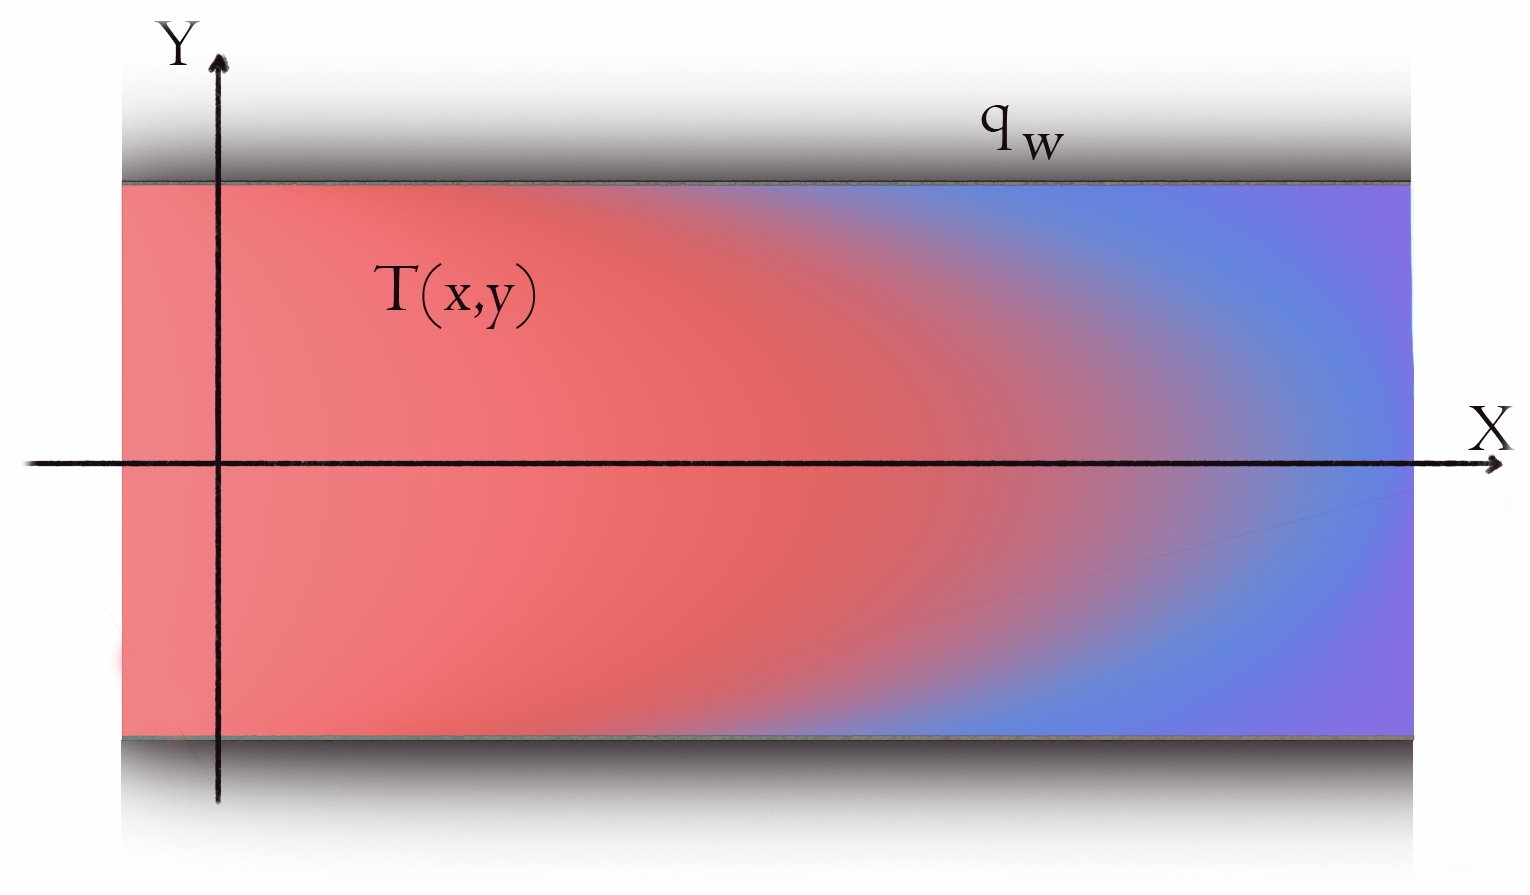
\includegraphics[angle=0, scale=0.14]{imagemtermico}
				\caption{Graphical representation of the thermal domain of the system.}
				\label{temperatura}
			\end{figure}
			\end{minipage}
		\end{frame}
		
		
		
		
		
		
		\begin{frame}
		\frametitle{Developing the temperature difference in the main equation}
		\begin{equation}
		\begin{split}
		\frac{\partial ( \overline{T^\ast + T_w}  ) }{\partial t} +
		\frac{\partial{}}{\partial{x}} \left(\overline{(T^\ast + T_w)^\prime u^\prime}\right) + \frac{\partial{}}{\partial{x}}\left(\overline{(T^\ast + T_w)} \ \overline{u}\right)+  \\
		\frac{\partial{}}{\partial{y}} \left(\overline{(T^\ast + T_w)^\prime v^\prime}\right) + \frac{\partial{}}{\partial{y}}\left(\overline{(T^\ast + T_w)} \ \overline{v}\right) = \\
		{\frac{\partial{}}{\partial{x}}} \left(\alpha {\frac{\partial{\overline{(T^\ast + T_w)}}}{\partial{x}}} \right) +
		{\frac{\partial{}}{\partial{y}}} \left(\alpha {\frac{\partial{\overline{(T^\ast + T_w)}}}{\partial{y}}} \right) .
		\end{split}
		\end{equation}
		\begin{center}\begin{equation}\begin{split}
		\frac{\partial ( \overline{ T^\ast + T_w } ) }{\partial t} +
		\frac{\partial{}}{\partial{x}} \left(\overline{T_w^{\prime} u^{\prime}}\right) +\frac{\partial{}}{\partial{x}} \left(\overline{{T^{\ast}}^{\prime} u^{\prime}}\right)
		+\frac{\partial{}}{\partial{x}}\left(\overline{u} \ \overline{T^{\ast}}\right)+ 
		\frac{\partial{}}{\partial{x}}\left(\overline{u} \ \overline{T_w}\right)+ 
		\\
		\frac{\partial{}}{\partial{y}} \left(\overline{{T^{\ast}}^{\prime} v^{\prime}}\right)+
		\frac{\partial{}}{\partial{y}} \left(\overline{T_w^\prime v^\prime}\right) + \frac{\partial{}}{\partial{y}}\left(\overline{v} \ \overline{T^\ast}\right) +
		\frac{\partial{}}{\partial{y}}\left(\overline{v} \ \overline{T_w}\right) 
		= 
		\\
		{\frac{\partial{}}{\partial{x}}} \left(\alpha {\frac{\partial{\overline{(T^\ast + T_w)}}}{\partial{x}}} \right) +
		{\frac{\partial{}}{\partial{y}}} \left(\alpha {\frac{\partial{\overline{(T^\ast + T_w)}}}{\partial{y}}} \right) .
		\end{split}\end{equation}\end{center}
		\end{frame}
		
		
		
		
		
%		\begin{frame}
%			\frametitle{Simplificações chave na velocidade}
%			$\bullet$ Para a velocidade, devem ser feitas as considerações de que é um sistema em regime permanente e unidimensional.
%			Assim, na equação da velocidade, teremos as seguintes simplificações:
%			\begin{equation}
%			\begin{split}
%			\color{red}\frac{\partial \overline{u}}{\partial t} \color{black}+\color{red} \frac{\partial \overline{u^2}}{\partial x} \color{black}+\color{red} \frac{\partial \overline{u} \ \color{blue}\overline{v}\color{red}}{\partial y}\color{black} + \color{red} \frac{\partial \overline{u} \ \color{blue}\overline{w}\color{red}}{\partial z} \color{black} =  - \frac{1}{\rho} \frac{\partial \overline{{p}}}{\partial x} + \frac{\partial}{\partial x} \left( \nu \color{red}\frac{\partial \overline{u}}{\partial x} \color{black} - \overline{{u^\prime}^2}\right) + \frac{\partial}{\partial y} \left( \nu \frac{\partial \overline{u}}{\partial y} - \overline{{u^\prime  v^\prime}}\right) \\
%			+ \color{red}\frac{\partial}{\partial z} \left( \nu  \frac{\partial \overline{u}}{\partial z} - \overline{ u ^\prime w ^\prime} \right) \color{black}
%			\end{split}
%			\end{equation}
%			\begin{equation}
%			\frac{1}{\rho} \frac{\partial \overline{p}}{\partial x} = \frac{\partial}{\partial y} \left( \nu \frac{\partial \overline{u}}{\partial y} - \overline{u^\prime v^\prime}\right)  
%			\end{equation}
%		\end{frame}
		
		
		
		
		
		\begin{frame}
		\frametitle{Key simplifications}
		$\bullet$ For the temperature, it was considered a permanent regime, the self similarity was considered too on the $x$ axis, besides that the wall temperature was considered stable, that is, without fluctuations.
	 	\begin{center}
	 	\begin{equation*}
	 		\begin{split}
	 		\color{red}\frac{\partial ( \overline{ T^\ast + T_w } ) }{\partial t} \color{black} +
	 		\frac{\partial{}}{\partial{x}} \left(\overline{ \color{red}T_w^{\prime} \color{black} u^{\prime}}\right) +
	 		\color{red}\frac{\partial{}}{\partial{x}} \left(\overline{{T^{\ast}}^{\prime} u^{\prime}}\right)+ \color{black}
	 		\color{red} \frac{\partial{}}{\partial{x}}\left(\overline{u} \ \overline{T^{\ast}}\right) \color{black}+ 
	 		\frac{\partial{}}{\partial{x}}\left(\overline{u} \ \overline{T_w}\right)+ 
	 		\\
	 		\frac{\partial{}}{\partial{y}} \left(\overline{{T^{\ast}}^{\prime} v^{\prime}}\right)+
	 		\frac{\partial{}}{\partial{y}} \left(\overline{\color{red}T_w^\prime \color{black} v^\prime}\right) + \frac{\partial{}}{\partial{y}}\left(\color{red}\overline{v} \color{black} \ \overline{T^\ast}\right) +
	 		\frac{\partial{}}{\partial{y}}\left(\color{red}\overline{v}\color{black} \ \overline{T_w}\right) 
	 		= 
	 		\\
	 		\color{red}{\frac{\partial{}}{\partial{x}}} \left(\alpha {\frac{\partial{\overline{(T^\ast + T_w)}}}{\partial{x}}} \right) \color{black}+
	 		{\frac{\partial{}}{\partial{y}}} \left(\alpha {\frac{\partial{\overline{(T^\ast + \color{red} T_w \color{black})}}}{\partial{y}}} \right) .
	 		\end{split}
	 	\end{equation*}
 		\end{center}
 		\begin{equation}\label{equation_var}
 			{\frac{\partial{}}{\partial{y}}} \left(\alpha {\frac{\partial{\overline{T^\ast}}}{\partial{y}}}   
 			- \left(\overline{ T^{\ast\prime} v^\prime}\right) \right)
 			= 
 			\overline{u}\frac{\partial{}}{\partial{x}}\left(\overline{T_w}\right)  .
 		\end{equation}
		\end{frame}
	
		
		
		
		
		
		\begin{frame}
			\frametitle{The Boussinesq hypothesis}
			$\bullet$ In this way, the turbulent flow had to be modeled. The term $\overline{T^{\ast\prime}  v^\prime}$ 
			can be developed according to the Boussinesq hypothesis, which postulates:
			\begin{equation}\label{bou}
			-\left(\overline{ u^\prime  v^\prime}\right) = 
			\nu_t \frac{\partial{\overline{u}}}{\partial{y}}
			\implies
			-\left(\overline{ T^{\ast\prime}  v^\prime}\right) = 
			\alpha_t \frac{\partial{\overline{T^\ast}}}{\partial{y}}.
			\end{equation}
			Thus, by developing the equation:
			\\
				\begin{equation}
				{\frac{\partial{}}{\partial{y}}} \left(\alpha {\frac{\partial{\overline{T^\ast}}}{\partial{y}}}   
				+ \alpha_t  \frac{\partial \overline{T^\ast}}{\partial y} \right)
				= 
				\overline{u}\frac{\partial{}}{\partial{x}}\left(\overline{T_w}\right) . 
				\end{equation}
		\end{frame}
	
	
	
	
		
		\begin{frame}
			\frametitle{The Prandtl mixing length}
			$\bullet$ Thus, arises the term of the turbulent thermal diffusion $\alpha_t$ that needs to be modeled. A new variable should be introduced, the turbulent Prandtl number, as follows:
			\begin{equation}
				Pr_t = \frac{\nu_t}{\alpha_t}.
			\end{equation} 
			So we have the $ \ nu_t $ value that needs to be modeled. The value of the turbulent Prandtl number of $ Pr_t = 0.71 $ that has been used in the literature.
			With the model of the Prandtl mixing length, it is postulated that:
			\begin{equation}
			\nu_t = {l_m}^2 \left| \frac{\partial \overline{u}}{\partial y} \right|.
			\end{equation}
		\end{frame}
		
		
		
		
		
		\begin{frame}
			\frametitle{Replacing the mixing length in the main equation}	
			$\bullet$ 
			The mixing length introduces a module into the differential model and the parameter of the turbulent Prandtl number.
			\\
				\begin{equation}
				{\frac{\partial{}}{\partial{y}}} \left( \left( \alpha   
				+ \frac{\nu_t}{Pr_t} \right) \frac{\partial \overline{T^\ast}}{\partial y} \right)
				= 
				\overline{u}\frac{\partial{}}{\partial{x}}\left(\overline{T_w}\right)  .
				\end{equation}
			\begin{equation}
			{\frac{\partial{}}{\partial{y}}} \left( \left( \alpha   
			+ \frac{{l_m}^2 \left| \frac{\partial \overline{u}}{\partial y} \right|}{Pr_t} \right) \frac{\partial \overline{T^\ast}}{\partial y} \right)
			= 
			\overline{u}\frac{\partial{}}{\partial{x}}\left(\overline{T_w}\right)  .
			\end{equation}
		\\
		
		It is possible to notice, when analyzing the dynamic domain, that for positive values of $ y $ the first derivative of velocity will always be negative, since by the principles of Dirichlet and Neumman, we have a velocity that decreases with the increase of $ y $. So we have: \\
			\begin{equation}
			{\frac{\partial{}}{\partial{y}}} \left( \left( \alpha   
			- \frac{{l_m}^2}{Pr_t}\frac{\partial \overline{u}}{\partial y} \right) \frac{\partial \overline{T^\ast}}{\partial y} \right)
			= 
			\overline{u}\frac{\partial{}}{\partial{x}}\left(\overline{T_w}\right)  .
			\end{equation}
		\end{frame}	
	
	
	
	
		\begin{frame}
			\frametitle{A model for the Prandtl mixing length}
			A model for $ l_m $ must be established. For this, we observed the experimental studies of Nikuradse, with which this parameter was modeled as follows.
			\begin{equation}
			L\left(\frac{y}{R}\right) = \frac{l_m}{R} = 0.14 - 0.08 \left(\frac{y}{R}\right)^2 - 0.06\left(\frac{y}{R}\right)^4.
			\end{equation}
			To further enrich the model, Cebeci and Bradshaw added the Van Driest damping function:
			\begin{equation}
			L\left(\frac{y}{R}\right)  = \frac{l_m}{R} = \left(\frac{l_m}{R} = 0.14 - 0.08 \left(\frac{y}{R}\right)^2 - 0.06\left(\frac{y}{R}\right)^4\right)\left\{  1 - e^{[(\tilde{y} - 1) \frac{Re_\tau}{26}]}\right\}.
			\end{equation}
			Thus, we have the mixing length defined by:
			\begin{equation}
			lm = L R.
			\end{equation}
			Being $ L $ a function in the $ y $ axis. It is important to note that at this  point the Cebeci constant was introduced.
			\begin{equation}
			{\frac{\partial{}}{\partial{y}}} \left( \left( \alpha   
			- \frac{{L}^2 R ^2}{Pr_t}\frac{\partial \overline{u}}{\partial y} \right) \frac{\partial \overline{T^\ast}}{\partial y} \right)
			= 
			\overline{u}\frac{\partial{}\left(\overline{T_w}\right)  }{\partial{x}}.
			\end{equation}
		\end{frame}
		
		
		
		
		
%		\begin{frame}
%			\frametitle{Desenvolvendo a equação dinâmica}
%			$\bullet$ Desenvolvendo a equação dinâmica foi possível se explicitar de forma exata a primeira derivada da velocidade.
%			\begin{equation}
%			\int \frac{1}{\rho} \frac{\partial \overline{p}}{\partial x} dy = \int \frac{\partial}{\partial y} \left( \nu  \frac{\partial \overline{u}}{\partial y} - {L}^2 R ^2 \left(\frac{\partial \overline{u}}{\partial y}\right) ^ 2 \right) dy  
%			\end{equation}
%			\begin{equation}
%			\frac{1}{\rho} \frac{\partial \overline{p}}{\partial x} \int 1 dy = \int \frac{\partial}{\partial y} \left( \nu  \frac{\partial \overline{u}}{\partial y} - {L}^2 R ^2 \left(\frac{\partial \overline{u}}{\partial y}\right) ^ 2 \right) dy  
%			\end{equation}
%			\begin{equation}
%			y \frac{1}{\rho} \frac{\partial \overline{p}}{\partial x} =  \nu  \frac{\partial \overline{u}}{\partial y} - {L}^2 R ^2 \left(\frac{\partial \overline{u}}{\partial y}\right) ^ 2 
%			\end{equation}
%			\begin{equation}
%			{L}^2 R ^2 \left(\frac{\partial \overline{u}}{\partial y}\right) ^ 2 - \nu  \frac{\partial \overline{u}}{\partial y} + y \frac{1}{\rho} \frac{\partial \overline{p}}{\partial x} = 0
%			\end{equation}
%			Observando-se a conformação em forma de polinômio de segundo grau, retirou-se as raízes, onde só uma delas teve consistência física.
%			\begin{equation}
%			\frac{\partial \overline{u}}{\partial y} = \frac{2 y \frac{1}{\rho}\frac{\partial \overline{p}}{\partial x} }{ \nu + \sqrt{\nu ^2 + 4 y \frac{1}{\rho} \frac{\partial \overline{p}}{\partial x} L ^2 R ^2}}
%			\end{equation}
%		\end{frame}
			
		
		
		
%		\begin{frame}
%		\frametitle{Modelo referente ao gradiente de pressão}
%		$\bullet$ Para este desenvolvimento se utilizou a definição da tenção cisalhante e uma análise segundo a primeira lei de Newton.
%		\begin{equation}
%		u_\tau = \sqrt{\frac{\left| \tau_w \right|}{\rho}}
%		\end{equation}
%		\begin{equation}
%		p_1 2R = 2 \tau_w \Delta x + p_2 2 R
%		\end{equation}
%		Assim, desenvolvendo e substituindo, temos:
%		\begin{equation}
%		\frac{\tau_w}{R} = \frac{(p_1 - p_2)}{\Delta x}
%		\end{equation}
%		\begin{equation}
%		- \frac{\partial \overline{p}}{\partial x} = \frac{\tau_w}{R} = \frac{u_\tau^2 \rho}{R} 
%		\end{equation}
%		\end{frame}
	
	
	
	
	
	
		\begin{frame}
			\frametitle{Nondimensionalization}
			$\bullet$ To compare this work with literature models more easily, the equation was Nondimensionalized with the constants according to wall coordinates. It was considered: $ \tilde{y} = \frac{y . Re_\tau}{R} $, $ \tilde{\overline{u}} = \frac{\overline{u}}{u_\tau} $ , $ \tilde{\overline{T}} = \frac{\overline{T}}{T_\tau} $ , $Re_\tau = \frac{u_\tau R}{\nu}$, $Pr_t = \frac{\nu_t}{\alpha_t}$, $Pr = \frac{\nu}{\alpha}$ e $T_\tau = \frac{q_w}{\rho C_p u_\tau}$, $\frac{\partial{\left(T_m\right)}}{\partial{x}} = \frac{q_w}{u_m  R \rho  C_p } $, $\frac{\partial \overline{p}}{\partial x} = - \frac{u_\tau^2 \rho}{R} $.
			\\
				\begin{equation}
				{\frac{\partial{}}{\partial{\tilde{y}}}} \left( \left( \frac{Re_\tau}{Pr}   
				- \frac{{L}^2 Re_\tau ^3}{Pr_t}\frac{\partial \tilde{\overline{u}}}{\partial \tilde{y}} \right) \frac{\partial \tilde{\overline{T^\ast}}}{\partial \tilde{y}} \right)
				= 
				\frac{\tilde{\overline{u}}}{\tilde{u_m}}.
				\end{equation}
		\end{frame}
	
	
	
		\begin{frame}
			\frametitle{The dynamic development}
			$\bullet$ 
			It is important to note how there is velocity in the main equation, that is, for the development of the thermal domain, the development of the dynamic channel profile was necessary. For this, a previously established RANS methodology was used, as follows:
				\begin{equation}
				\frac{\partial \tilde{\overline{u}}}{\partial \tilde{y}} = - \frac{2 \tilde{y} \frac{1}{Re_\tau} }{ 1 + \sqrt{ 1 + 4 L ^2 Re_\tau ^2 \tilde{y}}}.
				\end{equation}		
			In this way, we have the first derivative of velocity in an exact form.
		\end{frame}
	
	

	
	
	\section{Numeric model}
		
	
	
	
		
		\begin{frame}
			\frametitle{Discretization of space}
			\begin{minipage}[h!]{0.5\textwidth}
			$\bullet$ To discretize the space, an Eulerian domain was formulated. For the velocity a fourth-order Runge-kutta method was applied, while the temperature was arranged in a central differences scheme that had to be solved implicitly. The dynamic domain was solved first, and its numerical result were used in the development of the thermal profile. As for cell location, a cell center was determined on the wall, and a point between cells in the center of the channel, the rest of the space units being evenly distributed throughout the channel.
			\end{minipage}\hfill
			\begin{minipage}[h!]{0.45\textwidth}
			\begin{figure}
				\centering
				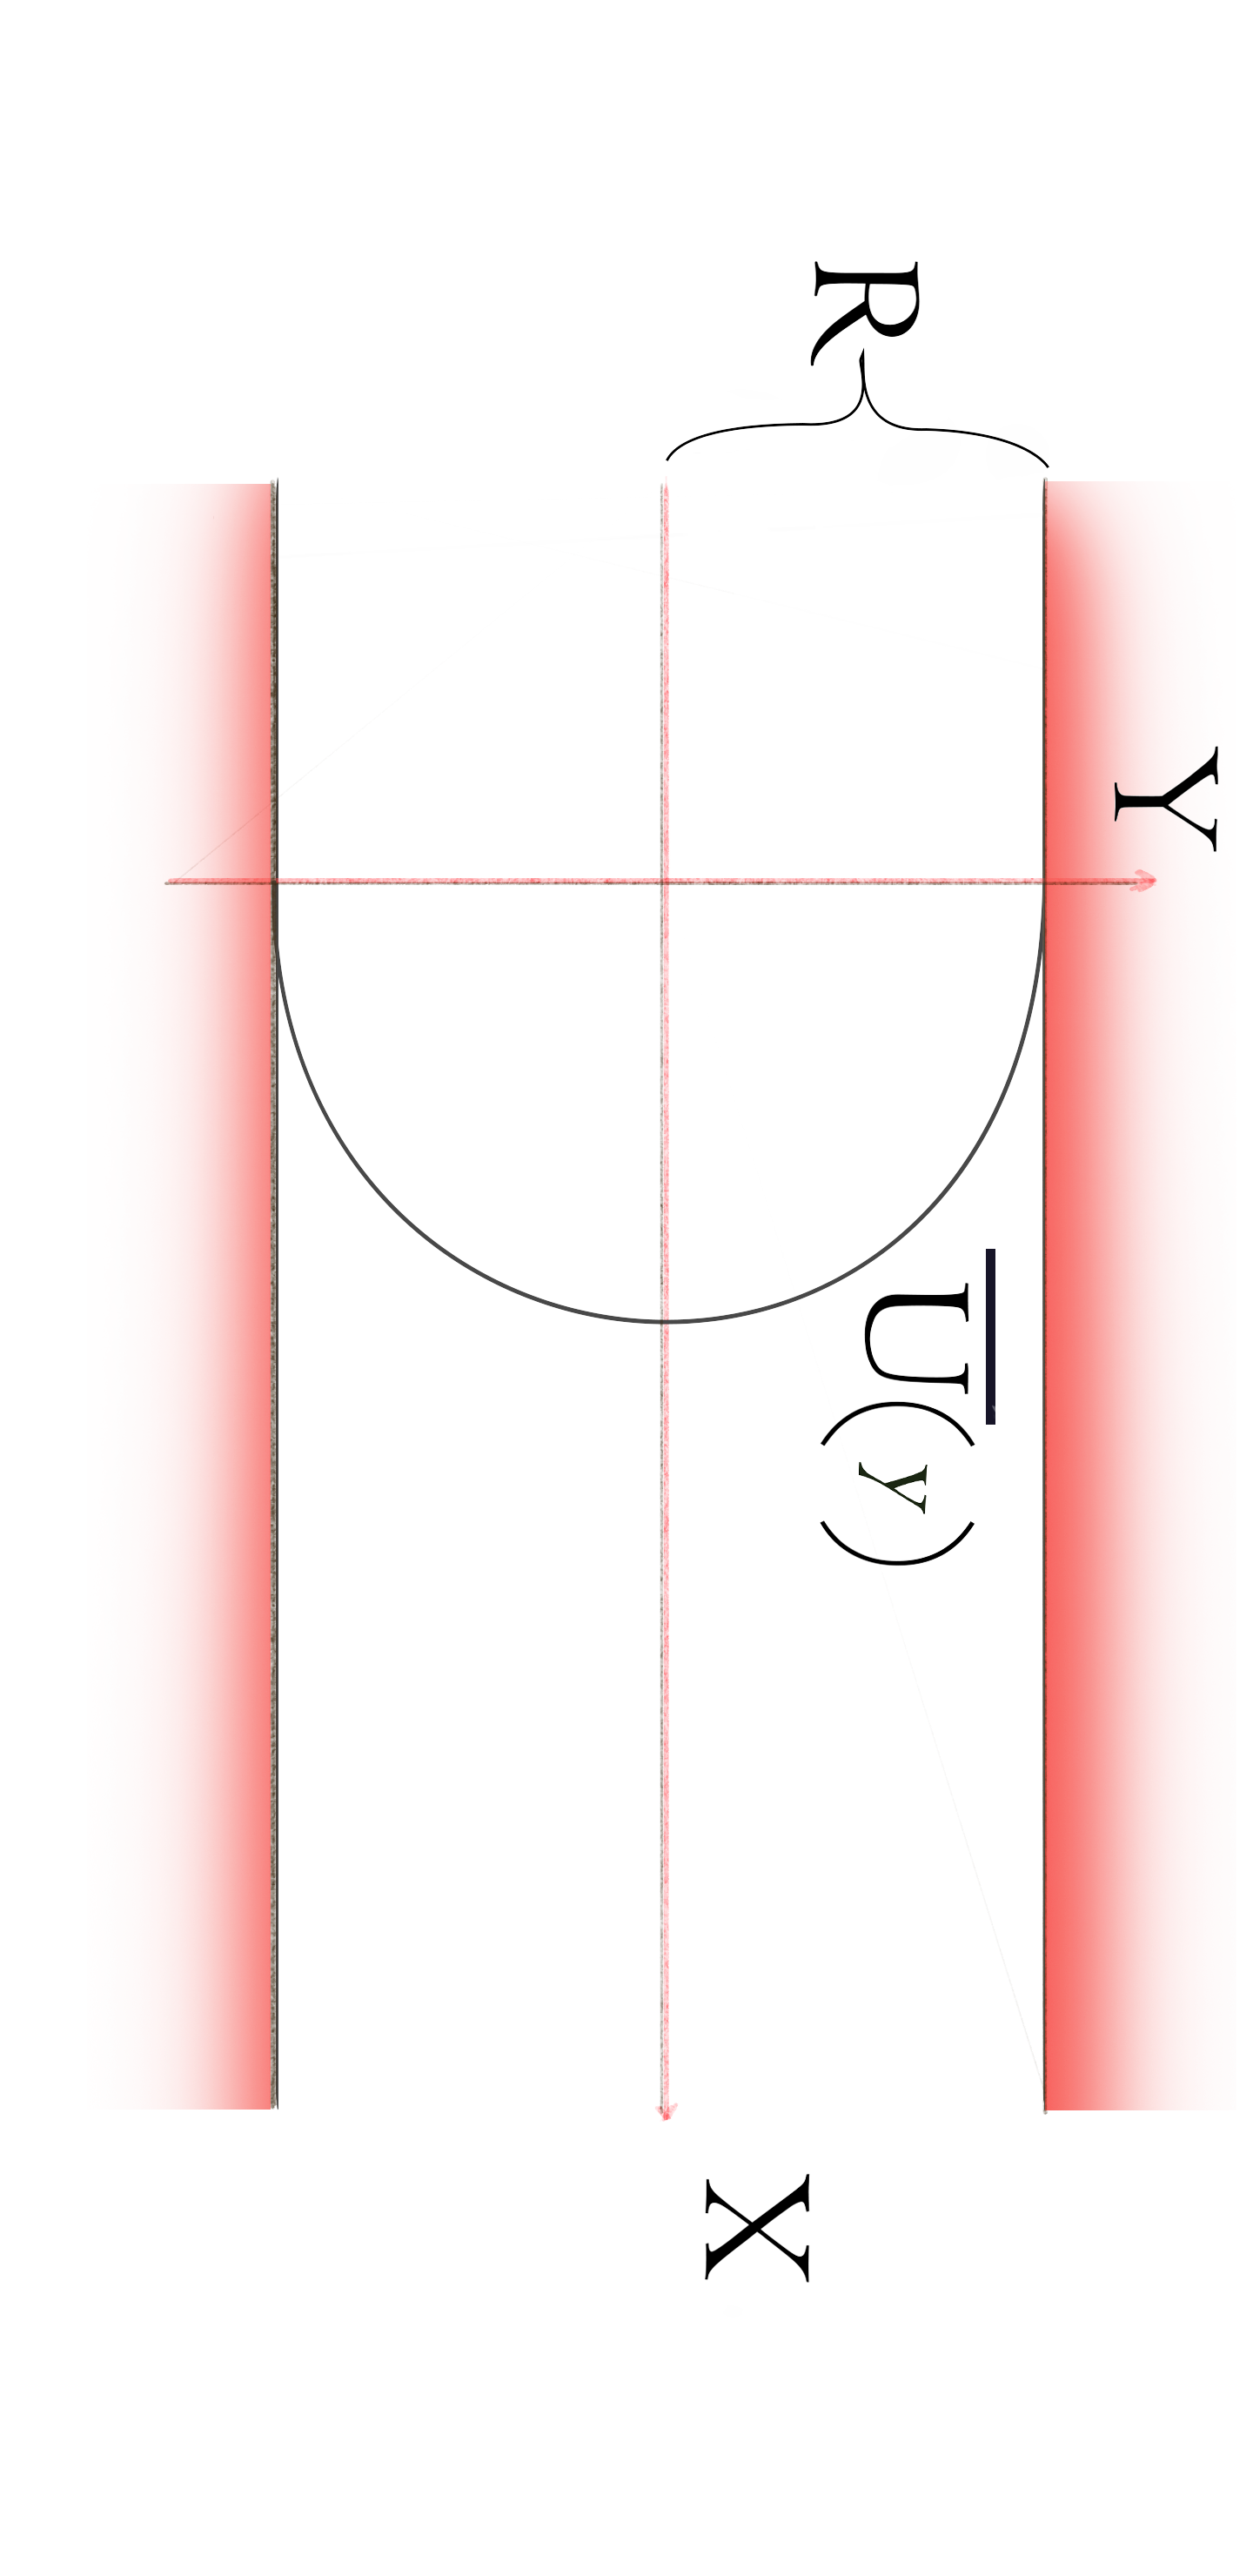
\includegraphics[angle=90, scale=0.06]{canalvermelho}
				\caption{Graphical representation of the system domain.}
				\label{sistema}
			\end{figure}
			\end{minipage}\\
		\end{frame}
	
	
	
	
	
			\begin{frame}
		\begin{figure}
			\centering
			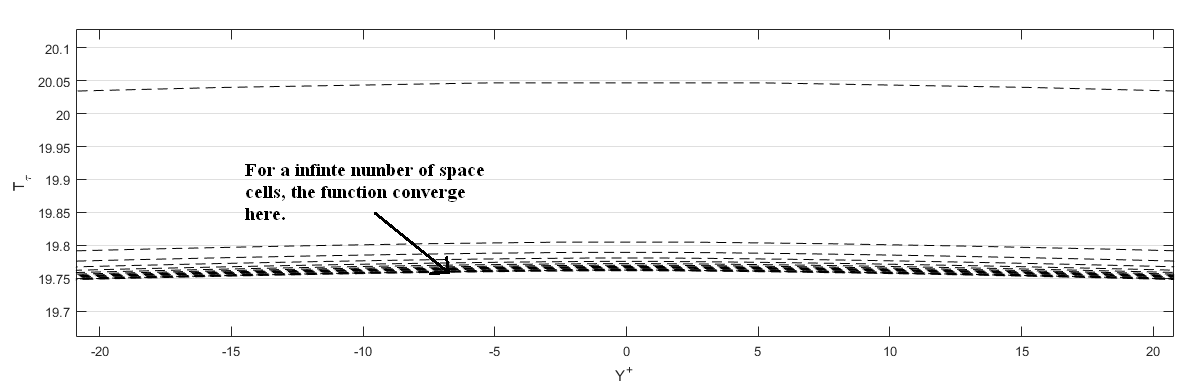
\includegraphics[angle=0, scale=0.32]{convergnciaprimeira}
			\caption{Convergence and net independence.}
			\label{convergencia}
		\end{figure}
	\end{frame}
		
	
	
	
		
	\section{Results}
		\begin{frame}
			\frametitle{Preliminary results: $Pr_t= 0.71$ , $A = 26 $}
				$\bullet$ Initially the turbulent Prandtl number was used as in the literature, a value of 0.71, where the results were:\\
			\begin{minipage}[h!]{0.5\textwidth}
			\begin{figure}
				\centering
				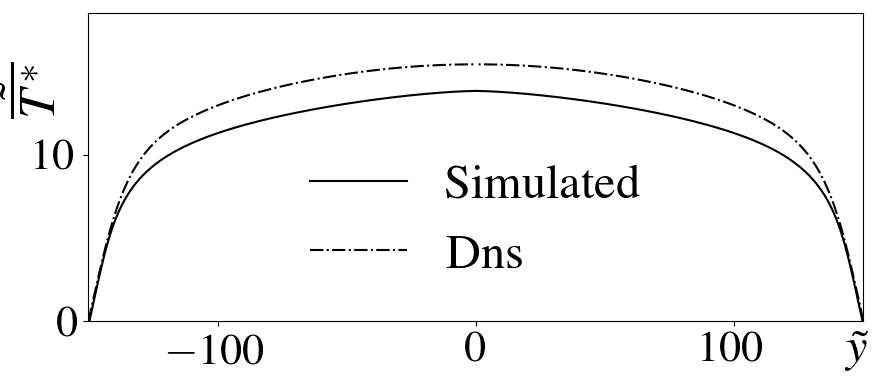
\includegraphics[angle=0, scale=0.24]{fotos_formatacao_final/Temperature_150_071_classico}
				\caption{Results for $Re_\tau = 150$. L2 = 1.42 }
			\end{figure}
			\end{minipage}
				\begin{minipage}[h!]{0.49\textwidth}
				\begin{figure}
					\centering
					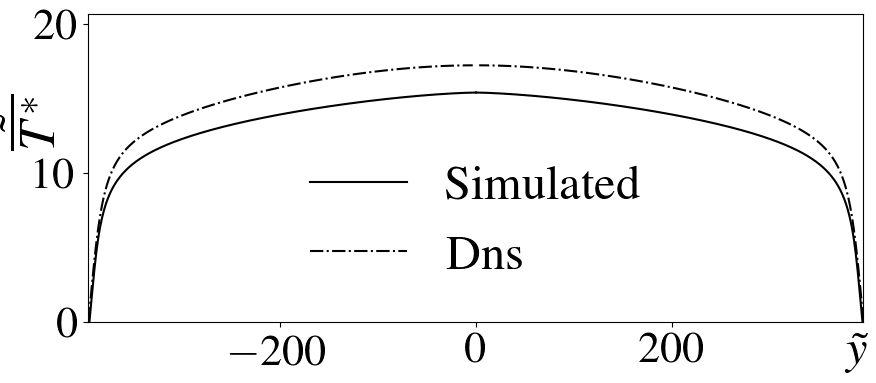
\includegraphics[angle=0, scale=0.24]{fotos_formatacao_final/Temperature_395_071_classico}
					\caption{Results for $Re_\tau = 395$. L2 = 1.55}
				\end{figure}
			\end{minipage}	\\
			\begin{minipage}[h!]{0.5\textwidth}
				\begin{figure}
					\centering
					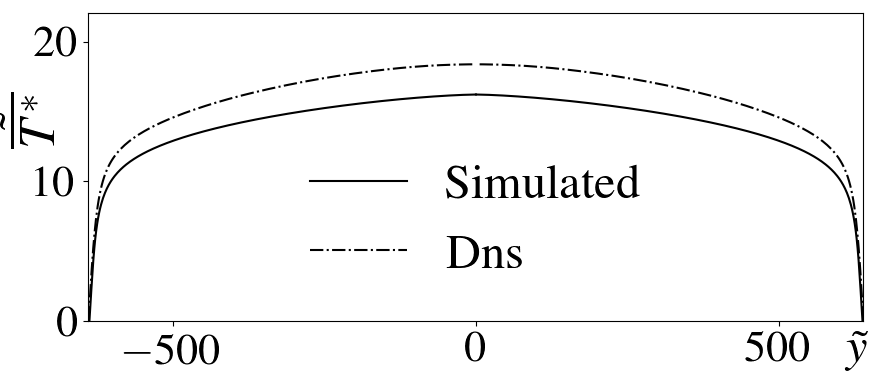
\includegraphics[angle=0, scale=0.24]{fotos_formatacao_final/Temperature_640_071_classico}
					\caption{Results for $Re_\tau = 640$. L2 = 1.79 }
				\end{figure}
			\end{minipage}
			\begin{minipage}[h!]{0.49\textwidth}
				\begin{figure}
					\centering
					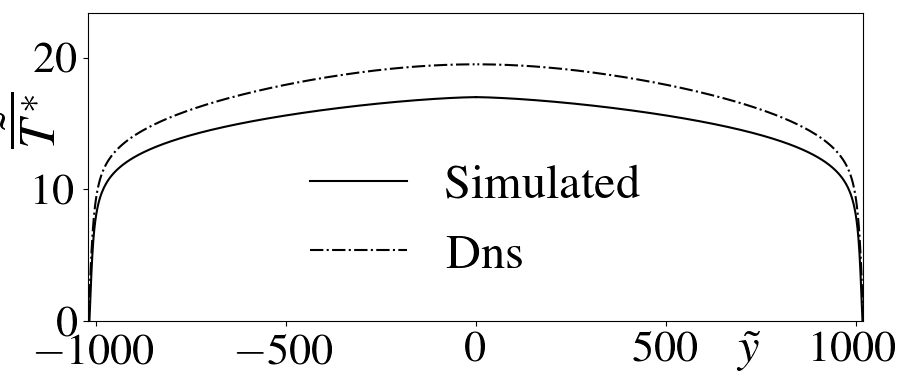
\includegraphics[angle=0, scale=0.24]{fotos_formatacao_final/Temperature_1000_071_classico}
					\caption{Results for $Re_\tau = 1020$. L2 = 2.04}
				\end{figure}
			\end{minipage}		
		\end{frame}
	
	
	
	
		
		\begin{frame}
		\frametitle{Study of the number of the turbulent Prandtl number provided by the DNS}
		\begin{minipage}[h!]{0.25\textwidth}
			$\bullet$ The result was observed for when the turbulent Prandtl number from the DNS was used, obtaining an L2 norm of $ 0.19 $ to $ Re_t = 640 $. Thus it was identified that the problem was in the parametrization of the turbulent Prandtl number that became the focus of the research.
		\end{minipage}\hfill
		\begin{minipage}[h!]{0.1\textwidth}
		\end{minipage}
		\begin{minipage}[h!]{0.65\textwidth}
			\begin{figure}
				\centering
				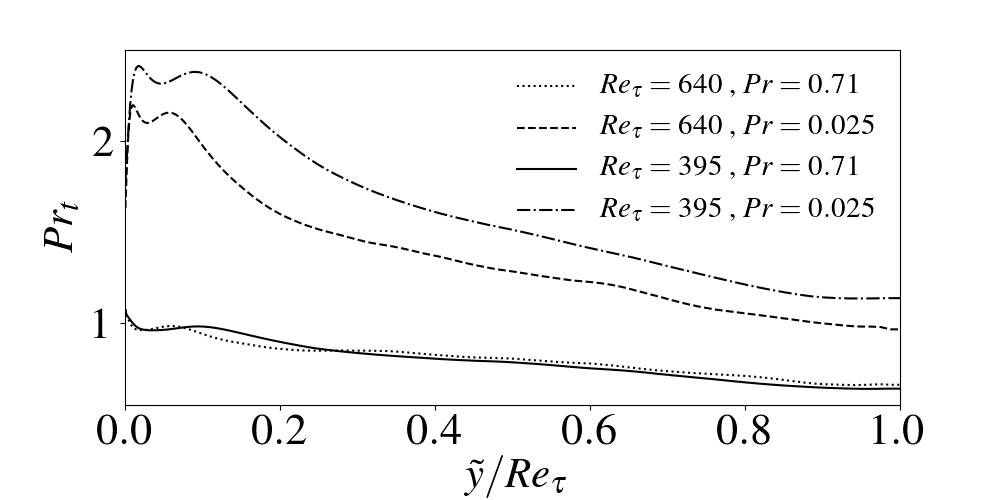
\includegraphics[angle=0, scale=0.30]{fotos_formatacao_final/DNS_PRt}
				\caption{DNS turbulent Prandtl number according to the coordinate $ y $ in the channel for various Reynolds numbers.}
			\end{figure}
		\end{minipage}	
		\end{frame}
	
	
		\begin{frame}
		\frametitle{The meta-modeling, with the genetic algorithm: Differential Evolution (DE)}
		\begin{minipage}[h!]{0.35\textwidth}
			$\bullet$ Was used an algorithm that searched for a minimal error for the function, considering the turbulent Prandtl number as an editable variable and the smaller error as the pattern of interest.
			
			It obtained a turbulent Prandtl number adjusted from $ 0.905 $ for the turbulent Reynolds number of $ 1020$.
			
			The value was applied to the entire domain.
		\end{minipage}
			\begin{minipage}[h!]{0.3\textwidth}
			\end{minipage}
			\begin{minipage}[h!]{0.55\textwidth}
			\begin{figure}
				\centering
				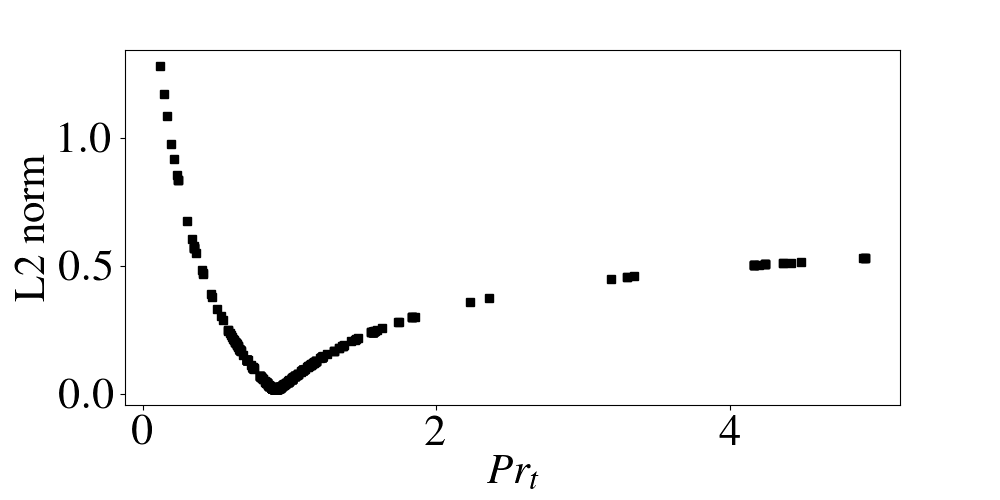
\includegraphics[angle=0, scale=0.3]{fotos_formatacao_final/Genetic_amostra}
				\caption{Scattering of samples from the Genetic optimization process. A convergence can be seen. This sample is from the optimization for the Reynolds number of 1020.}
			\end{figure}
		\end{minipage}	
		\end{frame}
		
		
		
		
		
		\begin{frame}
		\frametitle{Adjust of a fixed value: $Pr_t = 0.905$ , $A = 26$}
		$\bullet$Simulations with the turbulent Prandtl number set in $Re_\tau = 1020$:  \\
		\begin{minipage}[h!]{0.45\textwidth}
			 \begin{figure}
			 	\centering
			 	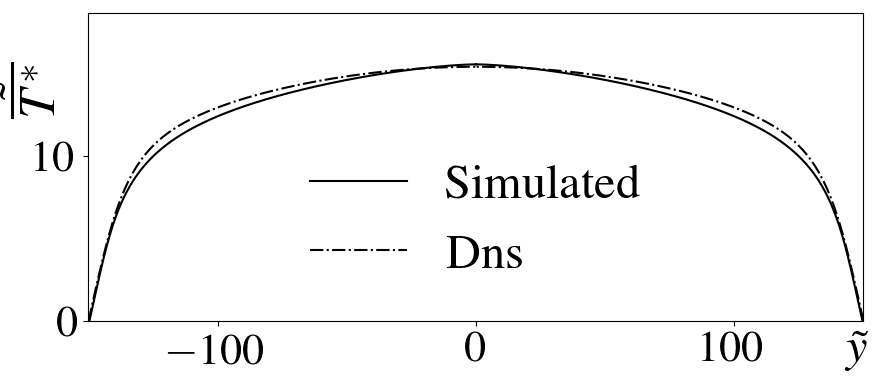
\includegraphics[angle=0, scale=0.18]{fotos_formatacao_final/Temperature_150_071_Prt0905_A26}
			 	\caption{Results for $Re_\tau = 150$. L2 = 0.26}
			 \end{figure}
			 \begin{figure}
			 	\centering
			 	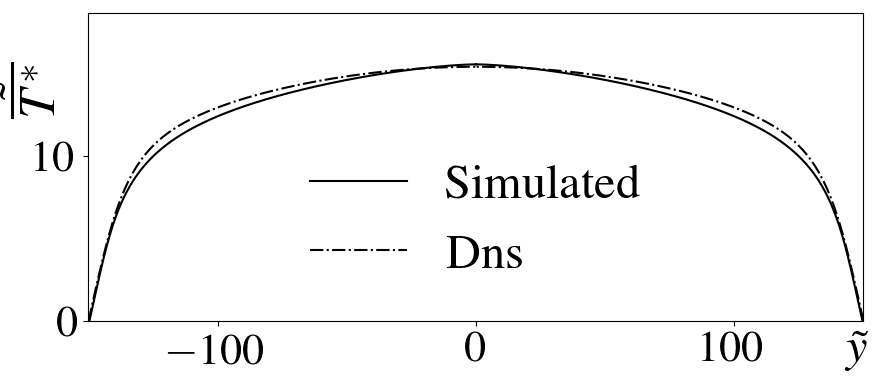
\includegraphics[angle=0, scale=0.18]{fotos_formatacao_final/Temperature_150_071_Prt0905_A26}
			 	\caption{Results for $Re_\tau = 395$. L2 = 0.22}
			 \end{figure}
		\end{minipage}\hfill
		\begin{minipage}[h!]{0.45\textwidth}
			\begin{figure}
				\centering
				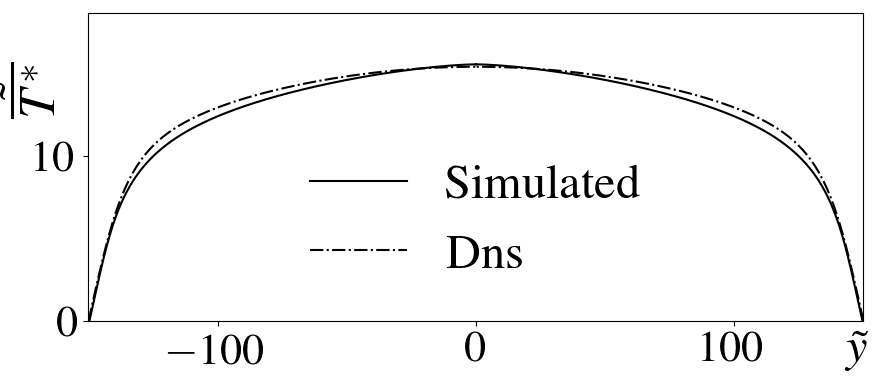
\includegraphics[angle=0, scale=0.18]{fotos_formatacao_final/Temperature_150_071_Prt0905_A26}
				\caption{Results for $Re_\tau = 640$. L2 = 0.174}
			\end{figure}
			\begin{figure}
				\centering
				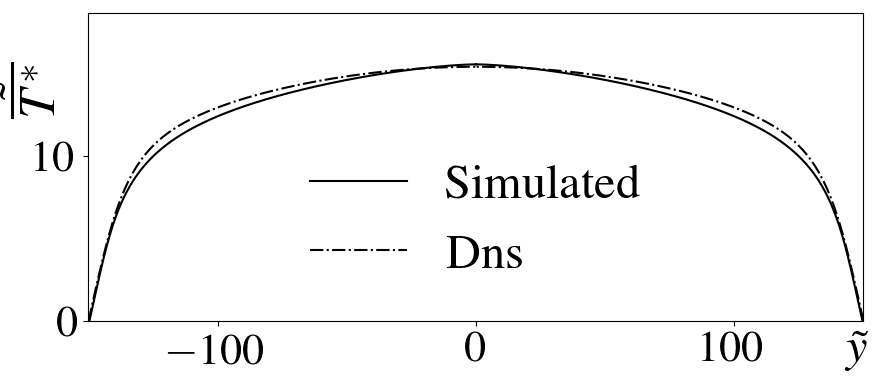
\includegraphics[angle=0, scale=0.18]{fotos_formatacao_final/Temperature_150_071_Prt0905_A26}
				\caption{Results for $Re_\tau = 1020$. L2 = 0.14}
			\end{figure}
		\end{minipage}		
		\end{frame}	
	
	
	
	
	
	
		\begin{frame}
		\frametitle{Optimization algorithm}
		$\bullet$ In order to obtain a curve that contemplated the Reynolds numbers throughout the domain, an optimizing algorithm was used to determine an ideal turbulent Prandtl number for each turbulent Reynolds number available in DNS.\\
		\begin{minipage}[h!]{0.5\textwidth}
			\begin{figure}
				\centering
				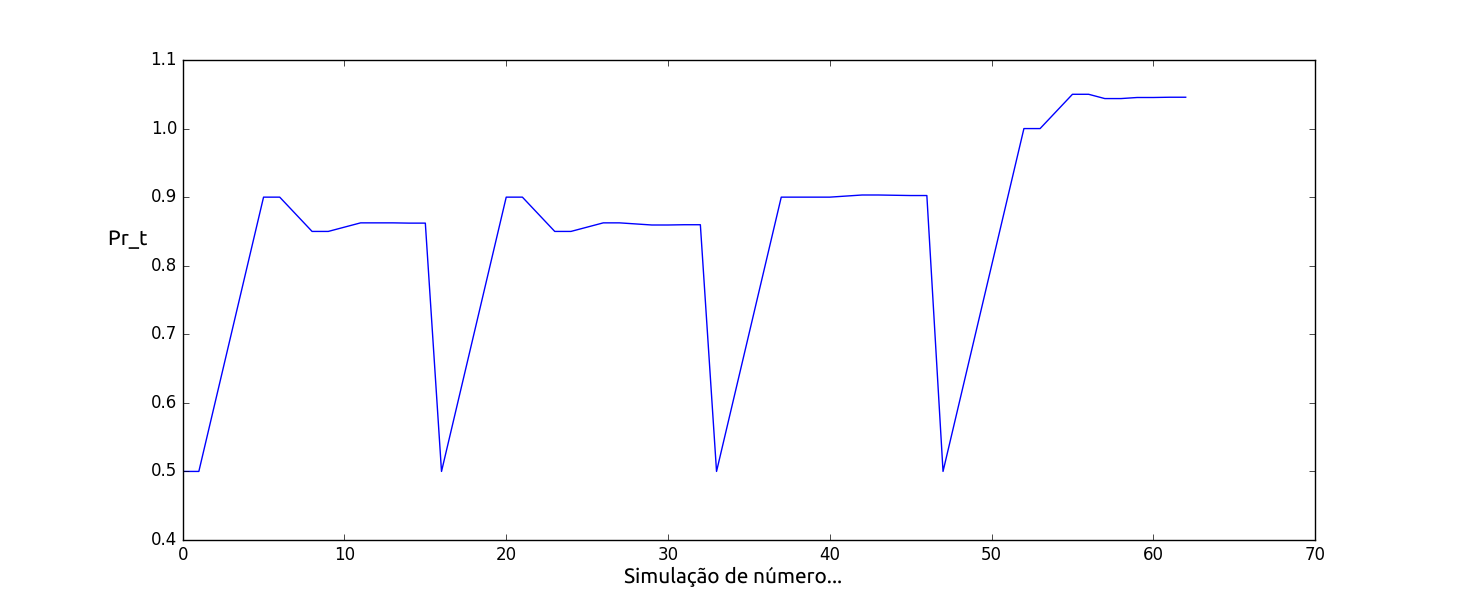
\includegraphics[angle=0, scale=0.18]{convergnciacima}
				\caption{Algorithm for optimal values. With initial value lower than the estimated.}
			\end{figure}
		\end{minipage}
		\begin{minipage}[h!]{0.45\textwidth}
			\begin{figure}
				\centering
				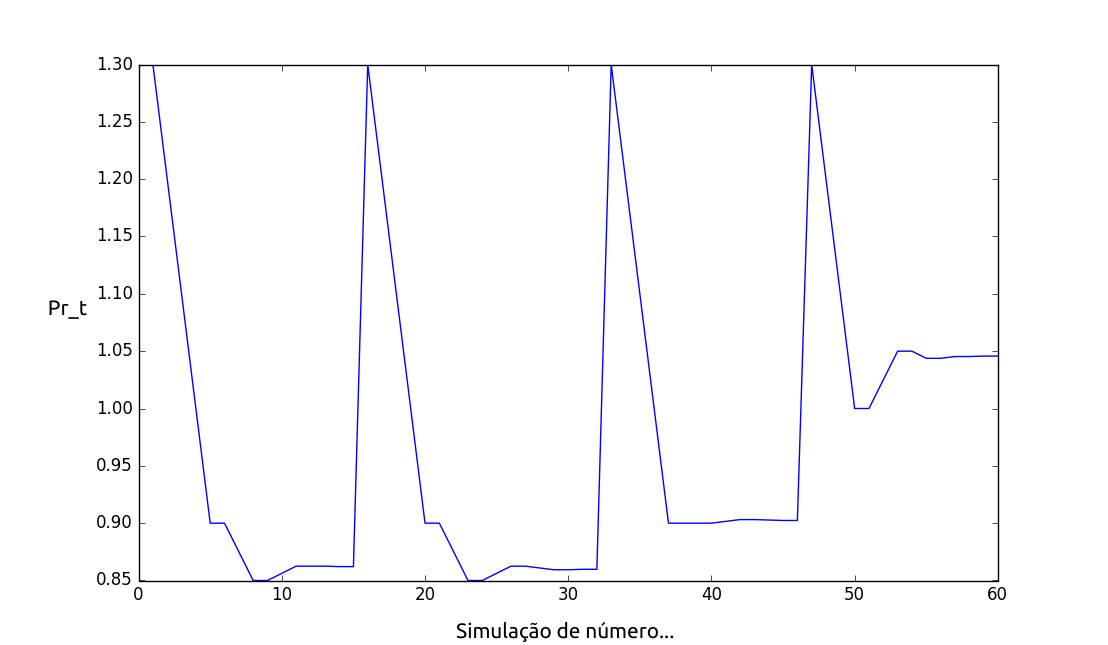
\includegraphics[angle=0, scale=0.22]{convergnciabaixo}
				\caption{Algorithm for optimal values. With initial value greater than the estimated.}
			\end{figure}
		\end{minipage}\\
	As a way of making sure that a global minimum has been reached, the algorithm was run from a point above and a point below the inferred.	
		\end{frame}
	
	
	
	
	
		\begin{frame}
		\frametitle{Adjust of the obtained values}
		\begin{minipage}[h!]{0.48\textwidth}
			$\bullet$ By performing a polynomial curve fit, the following relation was obtained:
			\begin{equation}
			\begin{split}
			Pr_t = 1,3 * 10^{-11} Re_\tau^3 - 7,1 * 10^{-8} Re_\tau^2 \\ + 0,0001 Re_\tau + 0,87 
			\end{split}
			\end{equation}
			Thus, a model adjusted for the turbulent Prandtl number as a function of the turbulent Reynolds number was developed.
		\end{minipage}
		\begin{minipage}[h!]{0.45\textwidth}
			\begin{figure}
				\centering
				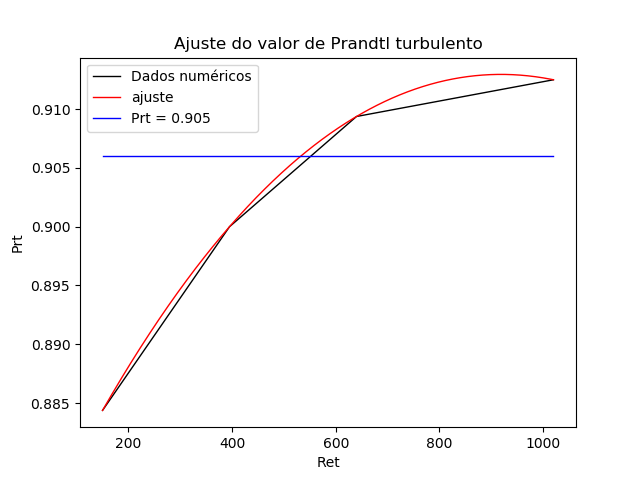
\includegraphics[angle=0, scale=0.43]{ajustePrandtl}
				\caption{Adjust of a model for the $ Pr_t $ variable.}
			\end{figure}
		\end{minipage}\\
		\end{frame}	
	
	
	
	
	
		\begin{frame}
		\frametitle{Adjust of the Cebeci's value}
		\begin{minipage}[h!]{0.45\textwidth}
			$\bullet$ From the resulting points of the optimization algorithm, the model adjusted for the Cebeci value was developed. As follows:
			\begin{equation}
			A = \frac{Re_\tau ^{0.0451 * \ln(Re_\tau)} *e ^ {5.2753} }{Re_\tau ^{0.6094}}
			\end{equation}
		\end{minipage}
		\begin{minipage}[h!]{0.51\textwidth}
			\begin{figure}
				\centering
				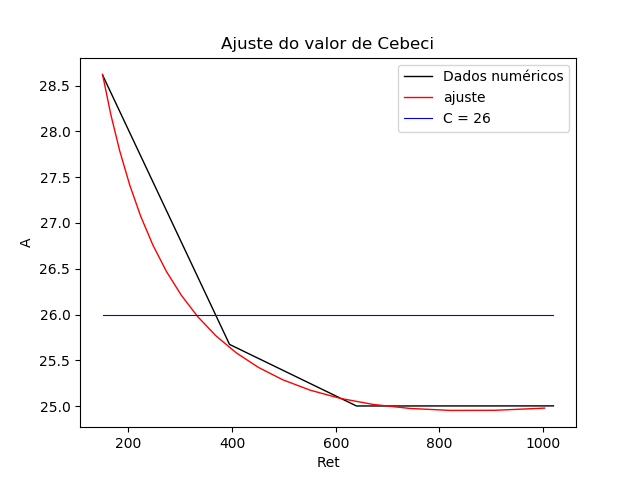
\includegraphics[angle=0, scale=0.45]{ajustecebeci}
				\caption{Adjust of a model for a variable Cebeci's number.}
			\end{figure}
		\end{minipage}
		\end{frame}	
	
	
	
	
	
		\begin{frame}
		\frametitle{Analysis of the influence of the Prandtl number}
		\begin{minipage}[h!]{0.45\textwidth}
			$\bullet$ It was studied the influence of the number of molecular Prandtl and it was observed that it was also a variable with influences in the error of the method, thus began a study with the objective of adding the influence of the value of Prandtl number to the parameterization of the turbulent Prandtl number. For this the following model was proposed:
		\end{minipage}
		\begin{minipage}[h!]{0.45\textwidth}
			\begin{figure}
				\centering
				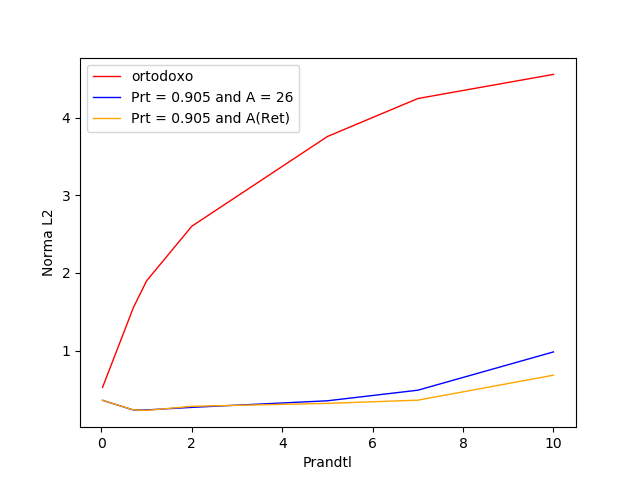
\includegraphics[angle=0, scale=0.42]{analisepr}
				\caption{Observation of the influence of Prandtl number.}
			\end{figure}
		\end{minipage}\\
		\begin{equation}
		\begin{split}
		Pr_t = \left( 1,3 * 10^{-11} Re_\tau^3 - 7,1 * 10^{-8} Re_\tau^2 + 0,0001 Re_\tau + 0,87 \right) \left(  \frac{Pr}{0,71}\right) ^{v}
		\end{split}
		\end{equation}
		\end{frame}
		
		
		
		
		
		
			\begin{frame}
		\frametitle{Genetic optimization algorithm}
		$\bullet$ In the adjustment of the exponent in the expansion of the parameterization of the turbulent Prandtl number, an evolutionary algorithm was used, which from an initial population of cases converged to the minimum error value.\\ 
		\begin{minipage}[h!]{0.32\textwidth}
			\begin{figure}
				\centering
				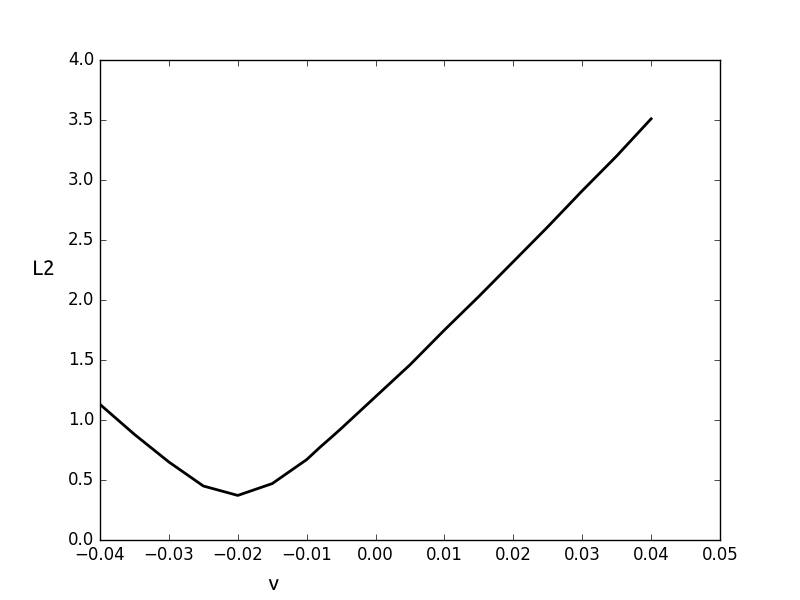
\includegraphics[angle=0, scale=0.19]{A100}
				\caption{Algorithm for optimal values, with mesh of 100 units.}
			\end{figure}
		\end{minipage}
		\begin{minipage}[h!]{0.32\textwidth}
			\begin{figure}
				\centering
				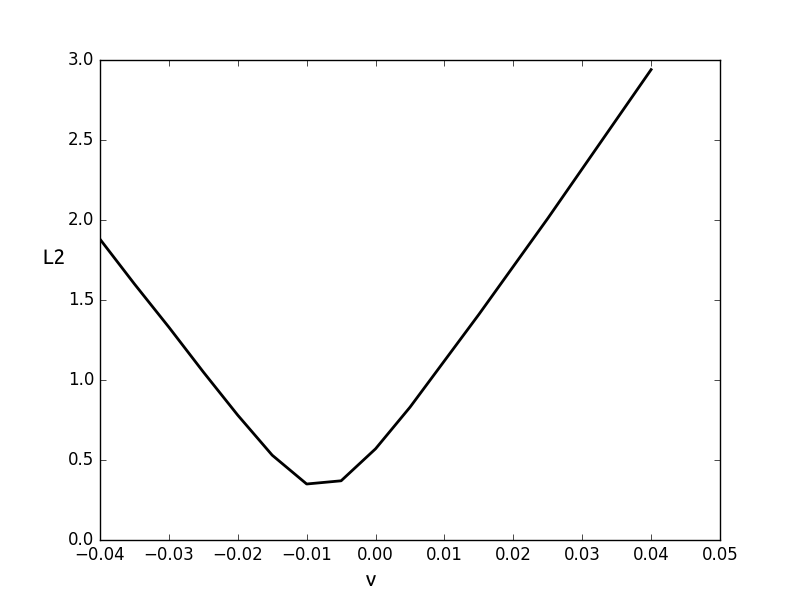
\includegraphics[angle=0, scale=0.19]{A400}
				\caption{Algorithm for optimal values, with mesh of 400 units.}
			\end{figure}
		\end{minipage}
		\begin{minipage}[h!]{0.32\textwidth}
			\begin{figure}
				\centering
				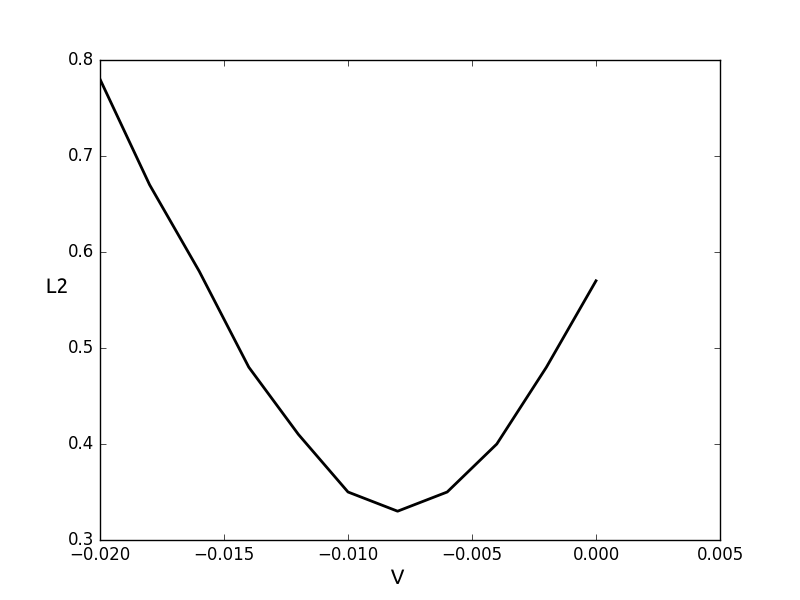
\includegraphics[angle=0, scale=0.19]{A400zoon}
				\caption{Algorithm for optimal values, with mesh of 400 units, advanced generation.}
			\end{figure}
		\end{minipage}	
		\begin{equation}
		\begin{split}
		Pr_t = \left( 1,3 * 10^{-11} Re_\tau^3 - 7,1 * 10^{-8} Re_\tau^2 + 0,0001 Re_\tau + 0,87 \right) \left(  \frac{Pr}{0,71}\right) ^{-0.008}
		\end{split}
		\end{equation}	
		\end{frame}	
	
	
	
	
	
%		\begin{frame}
%		\frametitle{General results}
%		\begin{center}
%			\animategraphics[trim = {1.7cm 2cm 0 1cm} , scale=1 , loop,controls = true, width=\linewidth]{10}{plot/plot_}{001}{180}
%		\end{center}
%		\end{frame}





\begin{frame}
\frametitle{Comparison between methods}
$\bullet$ Here are some cuts from the previous chart, explaining the errors obtained for a fixed Ret of 395, and a fixed Pr of 0.71.\\
\begin{minipage}[h!]{0.47\textwidth}
\begin{figure}
	\centering
	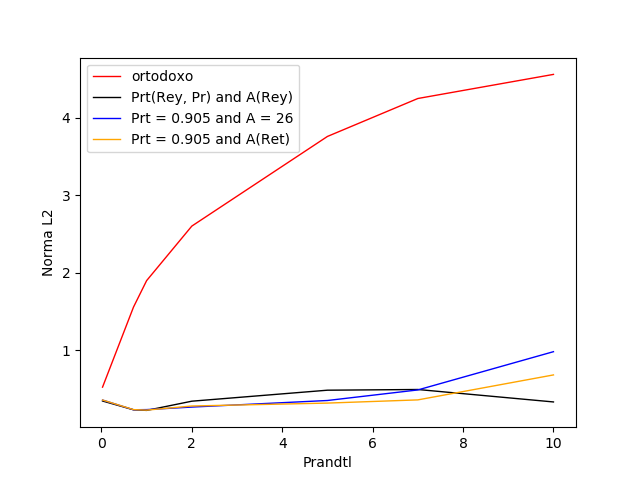
\includegraphics[angle=0, scale=0.39]{finaispr}
	\caption{Results for $Re_\tau = 395$}
\end{figure}
\end{minipage}
\begin{minipage}[h!]{0.47\textwidth}
\begin{figure}
	\centering
	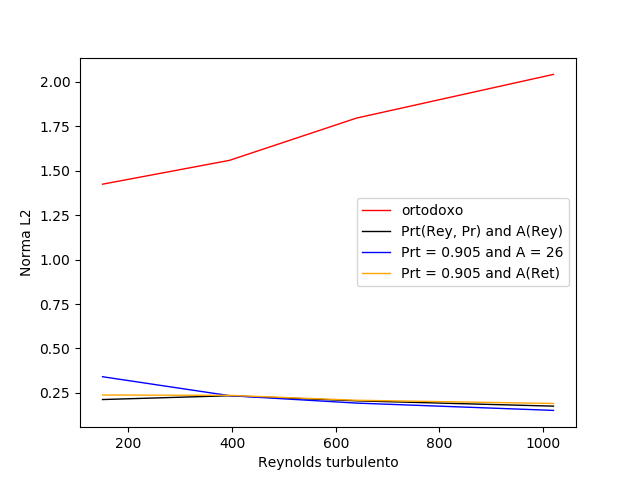
\includegraphics[angle=0, scale=0.39]{finaisRey}
	\caption{Results for $Pr = 0.71$}
\end{figure}
\end{minipage}\\
\end{frame}


	
	
	
	
	\section{Conclusion}
	
	
	
	
	
	
	
		\begin{frame}
		\frametitle{Conclusion}
		\begin{center}
		\begin{figure}
			\centering
			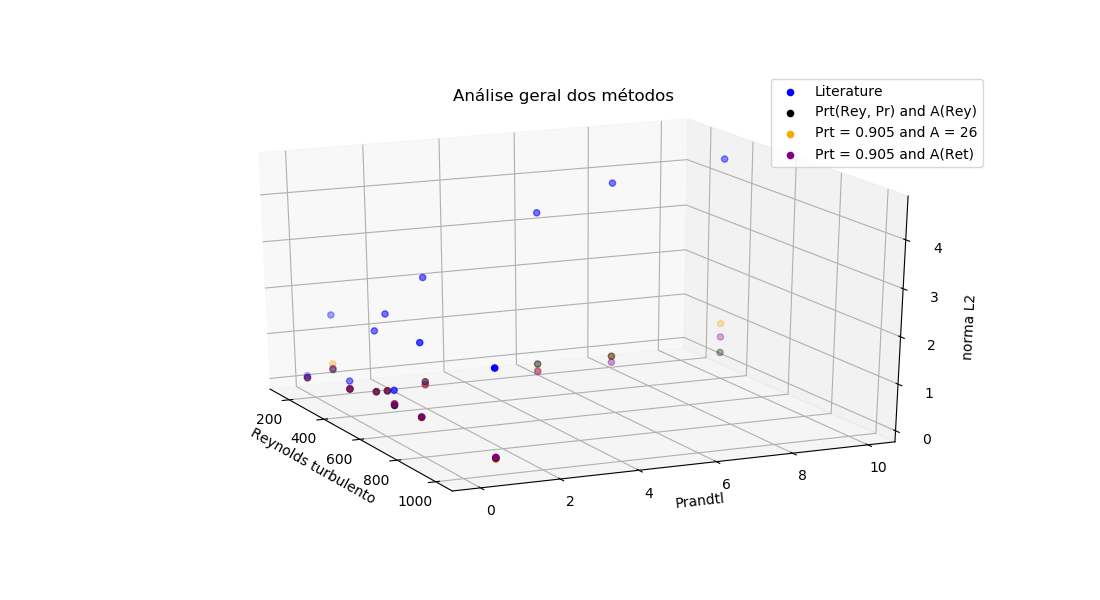
\includegraphics[angle=0, scale=0.42]{finais}
			\caption{Results.}
		\end{figure}
		\end{center}
		\end{frame}
			
		
		
		

	
	\section{Agradecimentos}
		
		
		
		
		
			\begin{frame}
				\placelogomflab 
				\frametitle{Agradecimentos}
				\begin{minipage}[h!]{0.4\textwidth}
			{
\includegraphics[trim=0.0cm 0.0cm 0.0cm 0.0cm,clip=true,height=0.25\textheight]{figuras/EPTT.jpg}}
				\end{minipage}
				\begin{minipage}[h!]{0.47\textwidth}
				\begin{figure}
					\begin{center}
						\begin{tabular}{c c}
							{
\includegraphics[trim=0.0cm 0.0cm 0.0cm 0.0cm,clip=true,height=0.2\textheight]{figuras/petrobras.png}}&{
\includegraphics[trim=0.0cm 0.0cm 0.0cm 0.0cm,clip=true,height=0.2\textheight]{figuras/logo_mflab.png}}\\
							{
\includegraphics[trim=0.0cm 0.0cm 0.0cm 0.0cm,clip=true,height=0.2\textheight]{figuras/cnpq.png}}&{
\includegraphics[trim=0.0cm 0.0cm 0.0cm 0.0cm,clip=true,height=0.2\textheight]{figuras/CAPES.png}}\\
							{
\includegraphics[trim=0.0cm 0.0cm 0.0cm 0.0cm,clip=true,height=0.2\textheight]{figuras/FAPEMIG.jpg}}&{
\includegraphics[trim=0.0cm 0.0cm 0.0cm 0.0cm,clip=true,height=0.2\textheight]{figuras/UFU_black.jpg}}\\
						\end{tabular}
					\end{center}
				\end{figure}
				\end{minipage}
			\end{frame}
			
			
			
			
			
			\begin{frame}
				\placelogomflab 
				\frametitle{Agradecimentos}
				\fontsize{44pt}{7.2}\selectfont
				\begin{center}
					Obrigado.
				\end{center}
			\end{frame}
		
		
		
		
\end{document}




		



%%%%%%%%%%%%%%%%%%%%%%%%%%%%%%%%%%%%%%% Exemplo de formatação de imagens		
%		\begin{frame}
%			\frametitle{Adição de fronteiras extras}
%			\begin{tabular}{c c}
%				
%				{\includegraphics[trim=0.0cm 0.0cm 0.0cm 0.0cm,clip=true,loop,height=0.5\textheight]{figuras/filtration_depois.png}}&{\includegraphics[trim=0.0cm 0.0cm 0.0cm 0.0cm,clip=true,loop,height=0.4\textheight]{figuras/filtration_depois_zoom.png}}\\
%				
%			\end{tabular}
%			
%		\end{frame}




%%%%%%%%%%%%%%%%%%%%%%%%%%%%%%%%%%%%%% Exemplo de formatação de imagens		
%		\begin{frame}
%			\frametitle{Agora}
%			\centering
%			\begin{tabular}{c}
%				
%				{\includegraphics[trim=0.00cm 2.0cm 0.0cm 2.0cm,clip=true,loop,width=0.9\textwidth]{figuras/t_x_51f.png}}\\{\includegraphics[trim=0.01cm 0.0cm 0.01cm 0.0cm,clip=true,loop,width=0.9\textwidth]{figuras/t_x_51999.png}}\\{\includegraphics[trim=0.01cm 0.0cm 0.01cm 0.0cm,clip=true,loop,width=0.9\textwidth]{figuras/t_x_51999g.png}}\\{\includegraphics[trim=0.01cm 0.0cm 0.01cm 0.0cm,clip=true,loop,width=0.9\textwidth]{figuras/t_x_51999y.png}}\\{\includegraphics[trim=0.01cm 0.0cm 0.01cm 0.0cm,clip=true,loop,width=0.9\textwidth]{figuras/t_x_51999b.png}}
%				
%			\end{tabular}
%			
%		\end{frame}





%%%%%%%%%%%%%%%%%%%%%%%%%%%%%%%%%%%%%  Formatação de equações:		
%		\begin{frame}
%			\frametitle{Newton-Raphson}
%			
%			\flushleft
%			Método de interface com jacobiano composto:
%			
%			\centering
%			\begin{equation}\label{forte_eqNewton}
%			K(D+\Delta D) \approx K(D)+\Delta D \, J(D)
%			\end{equation}
%			\begin{equation}\label{forte_eqNewton2}
%			K(D) =  Estrutura(Fluido(D))-D =  0
%			\end{equation}
%			\begin{equation}\label{forte_eqNewton3}
%			J(D) =  Estrutura'(Fluido(D)) \, Fluido'(D)-I
%			\end{equation}
%			\begin{equation}\label{forte_eqNewton4}
%			Fluido(D): \mathbb{R}^{n} \to \mathbb{R}^{m}
%			\end{equation}
%			
%			\flushleft
%			$Fluido'(D)$ é de tamanho $m x n$
%			
%			\centering
%			
%			\begin{equation}\label{forte_eqNewton5}
%			Estrutura(F): \mathbb{R}^{m} \to \mathbb{R}^{n}
%			\end{equation}
%			
%			\flushleft
%			$Estrutura'(F)$ é de tamanho $n x m$\\
%			$Estrutura'(Fluido(D)) \, Fluido'(D)$ e $I$ é de tamanho $n x n$
%		\end{frame}




%%%%%%%%%%%%%%%%%%%%%%%%%%%%%%%%%%%%%%%%%%% Vários exemplos de formatação textual:		


%		\begin{frame}
%			\frametitle{Conveniência do método de Multi Direct Forcing}
%			
%			\flushleft
%			\textbf{Fraco:}\\
%			$\bullet$ Predição da velocidade.\\
%			$\bullet$ MDF. (Imposição da condição de dirichlet na interface e cálculo da força)\\
%			$\bullet$ Estrutura.\\
%			$\bullet$ Poisson.\\
%			$\bullet$ Correção de velocidade e pressão.\\ \\
%
%			\textbf{Forte:}\\
%			$\bullet$ Predição da velocidade.\\
%			while \\
%			\quad	$\longrightarrow$ MDF.\\
%			\quad	$\longrightarrow$ Estrutura.\\
%			end\\
%			$\bullet$ Poisson.\\
%			$\bullet$ Correção de velocidade e pressão.\\
%
%		\end{frame}

		

%		
%%%%%%%%%%%%%%%%%%%%%%%%%%%%%%%%%  Modelo duas fotos lado a lado:


%		\begin{frame}
%		\frametitle{Limite do fraco}
%			ct=121
%			mi=200
%			\begin{tabular}{c c}
%			{\includegraphics[width=0.45\linewidth]{../../simulacoes_Estudo_dirigido2/fraco_mi_200_0_15_ct141/figuras/estrutura/vel_151}}&
%		   {\includegraphics[width=0.45\linewidth]{../../simulacoes_Estudo_dirigido2/fraco_mi_200_0_15_ct141/figuras/estrutura/vel_251}}\\
%		   {(a) Velocidade em linha centro da estrutura} & {(b) Velocidade transversal centro da estrutura}
%		\end{tabular}
%		\end{frame}



%%%%%%%%%%%%%%%%%%%%%%%%%%%%%%%%%%  Modelo tabela :

%		\begin{frame}
%			\frametitle{Comparação número de iterações}
%			\begin{tabular}{c c c c}
%				\hline
%				Método & Mínimo     &    Máximo &  Média\\ \hline
%				FPI MDF variável & 8     &    101 &  8.9764764764764760\\
%				FPI MDF fixo & 8     &     11 &  8.9099099099099099\\
%				QN Primeiro método de Broyden MDF variável & 18    &     101 &  18.281281281281281 \\ \hline
%			\end{tabular}
%		\end{frame}	




